% 中文报告正文（XeLaTeX 编译）
% 使用方法见 README.md；Overleaf 上编译引擎务必选 XeLaTeX
% ------------------------------------------------------------
\documentclass[11pt,a4paper]{ctexart}

% 页面与版式
\usepackage[margin=2.5cm]{geometry}
\usepackage{graphicx}
% 图片搜索路径：先找当前目录的 figures/，再找上一级目录的 figures/
% （main.tex 在 overleaf/ 里，figures/ 在项目根目录，所以用 ../figures/）
\graphicspath{{./figures/}{../figures/}}
\usepackage{booktabs}          % 三线表
\usepackage{amsmath}
\usepackage{array}
\usepackage{multirow}          % 表格里跨行合并单元格
\usepackage{hyperref}
\hypersetup{hidelinks}

% 中文字体：统一用 Fandol 字体集（ctex 自带的跨平台中文字体）。
% 这样做出来的 PDF 中文显示正常，选中复制、搜索、转 Word 也都能拿到正确文字；
% 否则 macOS 上 ctex 默认的 STKaiti / STFangSong 这类系统私有字体建立不出
% ToUnicode 映射，PDF 看着对、复制出来却是乱码。
% 若你的 TeX 发行版里没有 Fandol，把下面三行注释掉即可回退到系统默认中文字体。
\setCJKmainfont{FandolSong}[BoldFont={FandolSong-Bold}]
\setCJKsansfont{FandolHei}
\setCJKmonofont{FandolFang}

% 图表与正文的间距
\setlength{\intextsep}{0.5cm}
% 允许断行时适度拉伸字距，避免个别中英混排的长句顶出右边距（Overfull）
\tolerance=1500
\emergencystretch=1.5em

\title{河北十座光伏电站 15 分钟级功率预测：\\基线对比、机器学习方法评估与跨站迁移检验}
\author{徐敏纯\quad 学号 3120260807425}
\date{\today}

\begin{document}
\maketitle

% ============================================================
\section*{摘要}

光伏出力随天气起伏，电网需提前知道下一刻能发多少电。本文使用河北十座光伏电站的公开数据集 PVOD%
\cite{yao2021photovoltaic,pvod}（271968 条 15 分钟记录），回答两个问题：
复杂模型是否一定优于简单模型，以及如何更好地利用多站数据。

四种信息条件下比较朴素基线、线性回归、树模型与 LSTM：同时刻气象加历史观测时，
线性回归的 MAE 最低（1.4942\%，较基线降 41.74\%），优于全部树模型——
它能学到「出力$\approx$上一刻出力」的恒等映射，树模型只能输出分段常数；
换成预报气象则误差翻倍（4.8725\%）；LSTM 在四个设定上全部落后，
最差比线性回归差 111.6\%，耗时却高三千余倍。
留一站交叉验证中，多站联合训练是三类模型共同的最优做法
（LightGBM 降 14.61\%、XGBoost 降 4.11\%、LSTM 降 36.15\%），
预训练加微调只在可微的 LSTM 上有效（18.01\%），
直接搬用别站训好的模型则在三类模型上一律为负收益。

\noindent\textbf{关键词：}光伏功率预测；模型复杂度对比；恒等映射；皮尔逊相关分析；跨站迁移；留一站交叉验证

% ============================================================
\section{引言}

随着光伏装机容量的快速增长，出力的间歇性与波动性给电网调度带来压力，短时功率预测因此成为新能源并网的必要环节\cite{antonanzas2016review}。已有方法大致分三类：依据辐照度与组件温度推算出力的物理方法、依赖数值天气预报的统计方法，以及以随机森林、梯度提升树为代表的机器学习方法\cite{inman2013solar,sobroi2018review}。其中随机森林因对非线性关系拟合能力强、不易过拟合，在超短期预测中被广泛采用\cite{yang2021improved}；
以数值天气预报为输入的多种机器学习方法亦已有系统性横向对比\cite{markovics2022comparison}。

已有研究多默认「预测时刻的气象观测已可获得」。但实际情形并不统一：有的电站配有站内气象站，能拿到当前时刻的实测辐照；有的只能拿到数值天气预报；还有的既无实时气象采集、也无预报接入，只能依据已经采集到的历史序列外推当前出力。这三种信息条件下，模型能发挥多大作用、又分别在哪些天气条件下失效，尚缺乏在同一条流水线上、用长时段实测数据做的对照。

另一个容易被忽略的前提是：绝大多数研究只针对单一电站建模，结论是否适用于同一数据集之外的其他电站，很少被检验。而新建电站往往只有几周数据，恰是最需要预测、又最缺数据的场景。若能借助已运行电站的数据改善本站预测，其工程价值不亚于换一个更好的算法。

综合以上，本文围绕两个研究问题展开。

\textbf{研究问题一：复杂模型是否一定优于简单模型？}
在同一份数据、同一条时间切分下，把朴素基线（固定系数公式、Persistence）、
线性回归、随机森林、梯度提升树、XGBoost、LightGBM 与 LSTM 放在一起比较，
同时报告精度与训练耗时，看模型变复杂是否真的换来更低的误差。

\textbf{研究问题二：如何更好地利用多个站点的数据进行预测？}
用留一站交叉验证检验「借用别站数据」能否改善本站预测，
比较从零训练、预训练后微调、零样本迁移与多站联合训练四种做法，
并分别用树模型与 LSTM 各做一遍，观察两类模型是否遵循同一条规律。

为回答这两个问题，本文把「气象信息可得性」设为控制变量，
在四种信息条件下逐一复现：同时刻站内实测气象可得、同时刻仅有数值天气预报、
仅历史观测可用、以及同时刻气象与历史观测兼有；
再用特征重要性与特征消融解释模型到底依赖了什么，
最后对一个更基础的疑问作出检验——所用数据集的目标列是否为真实计量值。
全部实验在河北十座光伏电站的公开数据集 PVOD 上完成，
该数据集附完整元信息，且其目标列经检验为真实计量值（见 \ref{sec:targetcheck} 节）。

除精度之外，本文在分析过程中还发现了两件与数据本身有关、值得记录的事：一是原始时间戳为世界时而非北京时间，若不换算，太阳位置与日内曲线全都会错；二是在「同时刻气象加历史观测」这一最有利条件下，表现最好的竟是线性回归而非任何树模型。前者属于数据质量检查，后者需要给出机制解释，二者分别在 \ref{sec:quality} 节与 \ref{sec:identity} 节交代。

% ============================================================
\section{数据与方法}
% ------------------------------------------------------------
\subsection{数据说明}
\label{sec:data}

本文使用公开数据集 PVOD（Photovoltaic Output Dataset），含河北十座光伏电站的运行记录，
共 271968 条、15 分钟粒度，时间跨度自 2018 年 6 月 30 日至 2019 年 6 月 13 日，
并附有装机容量、经纬度、阵列倾角、组件型号等元信息\cite{yao2021photovoltaic,pvod}。

该数据集把气象变量分成两组：\texttt{nwp\_*} 共 7 项，为数值天气预报给出的预报值，含总辐射、
直接辐射、气温、相对湿度、风速、风向与气压；\texttt{lmd\_*} 共 6 项，为站内辐射计与气象仪的
实测值，含总辐射、散射辐射、气温、气压、风速与风向。预测目标为电站输出功率，单位 MW。

十座电站的装机容量相差数倍（6.6$\sim$35\,MW），功率绝对值无法直接比较，
故目标统一归一化为「功率/装机容量」，误差单位记作 \%装机容量，跨站可比。

关于数据取舍需要说明一句。任务给定两个候选数据集，另一份为宁夏某光伏电站 2019 年数据
\cite{ningxia2019photovoltaic}。那份数据在预备实验中表现出两个难以处理的性质：其目标列与总辐射
的比值几乎恒定（变异系数仅 0.23\%），近似由辐射按固定系数换算而来，而非独立计量的电表读数；
同时其页面未公开经纬度与装机容量，无法完成容量归一化，也就无法与其他电站横向比较。
PVOD 的目标列经检验为真实计量值（见 \ref{sec:targetcheck} 节），且附完整元信息，故本文全部实验改用 PVOD。
这一取舍本身也是一项检验结果，而非便利性选择。

% ------------------------------------------------------------
\subsection{数据质量检查}
\label{sec:quality}

按行统计，271968 条原始记录中无任何缺失值；重复时间戳 1 条，已保留首次出现者。
剔除「总辐射为 0 却仍有出力」的夜间异常记录 165 条（0.061\%）后，共用 271803 条。
归一化出力的峰值在十站之间落在 0.602 至 1.338 区间，
其中 station04 达 1.338，即出力超出登记装机容量 33.8\%，应是容量登记错误；
station09 仅 0.602，出力长期偏低，疑似限发。这两站因此在后续解释结果时被单独指出。

除常规检查外，本文发现三处若不留神就会让实验失效的问题，逐条记录如下。

\textbf{（1）时间戳为世界时，不是北京时间。}
按原始时钟小时统计总辐射，其峰值出现在 4 时，而河北约在 115$^\circ$E$\sim$119$^\circ$E，
正午应在 12 时前后。换算为北京时间（+8 小时）后，峰值回到 12 时，日落与日出时刻也与纬度相符。
图 \ref{fig:timezone} 给出两支曲线的对比。若不换算，太阳位置、晴空指数、日内曲线与「白天」样本的
判定全都会错位 8 小时。本文全流程统一按北京时间处理。

\begin{figure}[htbp]
\centering
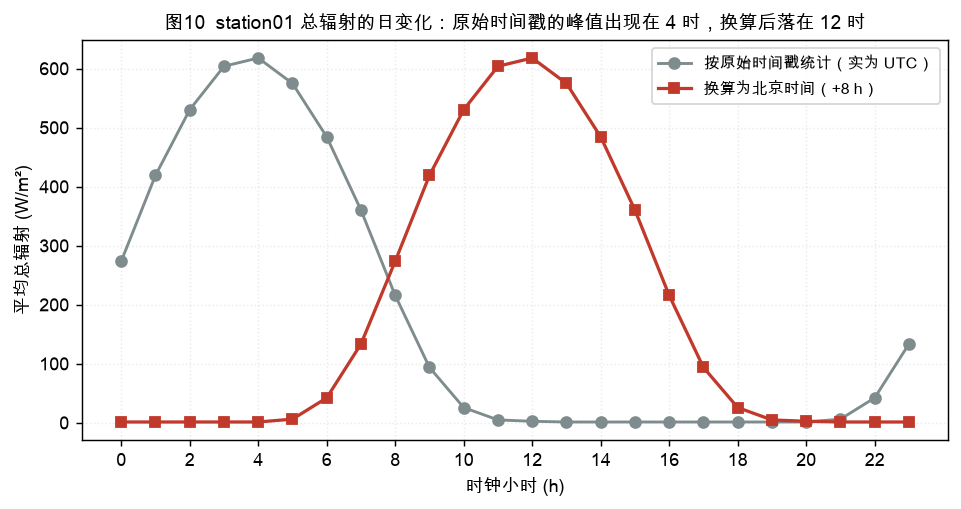
\includegraphics[width=0.8\textwidth]{fig10_timezone}
\caption{总辐射日变化：按原始时间戳统计的峰值出现在 4 时，换算为北京时间后落在 12 时}
\label{fig:timezone}
\end{figure}

\textbf{（2）时间序列存在天数级断点。}
十站合计出现 130 处非 15 分钟的间隔，最大一处跳了 6 天。这类断点对时序建模是致命的：
直接对功率做 \texttt{shift(1)} 时，断点后第一条记录取到的「上一刻」其实是数天前同一时刻的值，
滞后特征完全失真。本文因此不使用普通的 \texttt{shift}，而是先核对相邻记录的时间间隔，
间隔不等于 $k\times15$ 分钟者一律置为缺失，再由 \texttt{dropna} 整行剔除。
此外，测试集与训练集严格按时间先后切分、绝不打乱，以免相邻时段的天气模式跨越边界造成泄露。

\textbf{（3）存在「平顶」片段，疑似缺测被常数填充。}
station01 的 2019-06-10 最具代表性：10:00 至 19:00 总辐射恒为 837.80\,W/m$^2$，
功率恒为 14.03\,MW，曲线呈方波而非钟形。按「总辐射连续 8 个点（2 小时）以上完全相等且数值大于
100\,W/m$^2$」判定，十站合计 171 行属于此类（占 0.063\%），集中在 4 个站日。
占比很小，不足以影响整体结论，但足以在挑「典型日」画图时把人带偏，故本文在选取典型日时将其排除。

% ------------------------------------------------------------
\subsection{实验设定与评估指标}
\label{sec:setup}

为对应三种真实的信息可得性，本文设置三个设定。三者的预测目标都是同一时刻的电站出力，
差别只在输入可用什么。

\textbf{设定甲（同时刻站内实测气象）。}输入为预测时刻本身的站内实测读数，即 6 个 \texttt{lmd\_*} 变量，
叠加时刻正余弦编码 hour\_sin、hour\_cos、doy\_sin、doy\_cos，合计 10 个特征。
该设定对应「站内气象站实时可得」的现报场景。

\textbf{设定甲$'$（同时刻数值天气预报）。}输入换成 7 个 \texttt{nwp\_*} 变量加同样的 4 个时刻编码，
合计 11 个特征。它对应没有站内气象站、只能接入预报的电站。
把甲与甲$'$并列，能量化「预报误差」相比「站内实测」要让精度损失多少。

\textbf{设定乙（仅历史观测）。}剔除预测时刻自身的一切读数，只使用此前若干刻钟的观测：
上一刻及 2、3、6、12 刻钟前的总辐射，上一刻钟的功率，以及 1、6 刻钟前的气温，
再叠加同样的 4 个时刻编码，合计 12 个特征。该设定不存在数据泄露，对应「只能拿已采集数据估算当前出力」
的场景，是三者中条件最苛刻的。

\textbf{设定丙（同时刻气象 $+$ 历史观测）。}把甲与乙的输入合并：6 个 \texttt{lmd\_*} 变量、
上一刻功率、上一刻辐射，再加 4 个时刻编码，合计 12 个特征。加这一组是为了回答
「在已知上一刻功率之后，同时刻气象还能不能再贡献一点」——甲没有自回归项，直接与乙比较并不公平。

四个设定采用同一套时间切分：按时间先后划分，前 70\% 样本用于训练、后 30\% 用于测试，
训练与测试之间不打乱样本顺序。所有模型固定随机种子 \texttt{random\_state=42}，保证可复现。

预测性能用平均绝对误差 MAE、均方根误差 RMSE 与决定系数 $R^2$ 三项指标衡量，
单位均为 \%装机容量。另设两条不做学习的朴素基线作对照：设定甲与甲$'$采用由训练集
最小二乘拟合的固定系数公式 $P=k\cdot \mathrm{GHI}$，设定乙与设定丙采用 Persistence 基线，
即直接把上一刻钟的功率当作本刻钟的预测值。

参与比较的模型为线性回归、随机森林、梯度提升树 GBDT、LightGBM 与 XGBoost 五种。
为保证可比，四个树模型统一取 100 棵、学习率 0.1；随机森林取 200 棵（其原理见 \cite{breiman2001random}）。
调参过程有两点记录在案：一是 XGBoost 的库默认学习率是 0.3，在若干站上明显过拟合，
故另设一行「默认学习率」作为对照如实列出；二是树数并非越多越好，试过 300 棵后十站平均反而变差
（LightGBM 由 2.2821 升至 2.4538），说明本任务 100 棵已足够。

% ------------------------------------------------------------
\subsection{跨站迁移实验的设定}
\label{sec:transfersetup}

\ref{sec:setup} 节的四个设定都只用一座电站的数据训练。为回答「能否借用别站数据改善本站预测」，
本文在 PVOD 十站上做留一站交叉验证（Leave-One-Station-Out）：轮流把每一站当作待预测的目标站，
其余九站作为源数据，共跑十轮，使结论不受单个站的偶然性支配。每轮比较四种做法：

\begin{itemize}
  \item A 从零训练：只用目标站自己的训练数据。
  \item B 预训练 + 微调：先在其余九站上训练，再用目标站数据继续加树。
  \item C 零样本迁移：直接把九站模型套到目标站，完全不看目标站的任何标签。
  \item D 多站联合训练：九站与目标站数据混合训练，目标站样本权重放大 5 倍。
\end{itemize}

这里有一处公平性必须控制：B 的总树数是「500 棵预训练 $+$ 200 棵微调」，
因此 A 也取 700 棵，否则 B 的胜利可能只是「树更多」的胜利，而非迁移本身有效。
四种做法统一使用 LightGBM（后续 \ref{sec:xgb} 节会换 XGBoost 复跑一遍），
目标站内部仍按时间前 70\% 训练、后 30\% 测试。
输入特征为 6 个站内实测气象变量 $lmd\_*$ 加 6 个时刻/风向编码，
与 \ref{sec:overall} 节设定甲的口径一致（时间戳同样已换算为北京时间），
因此本节结果可与单站实验横向比较。

树模型的「微调」只是接着加树，已经长出来的老树一棵都改不掉。神经网络没有这个限制，
可以继续反向传播，所有权重都跟着变。这种差别会不会改变迁移的结论，值得单独验证。
因此本文用同一批数据、同一套清洗与切分，把上述实验又用 LSTM 做了一遍，方案与树模型一一对应，
另加一组对照：

\begin{itemize}
  \item A 从零训练：只用目标站自己的训练数据，训练 15 轮。
  \item B 预训练 + 微调：九站上预训练 10 轮，再用目标站数据以较小学习率微调 5 轮。
  \item C 零样本迁移：预训练完成后直接在目标站测试，不看目标站任何标签。
  \item D 多站联合训练：九站与目标站数据混合训练，目标站样本权重放大 5 倍。
  \item E 预训练初始化 + 训满：用预训练权重作初始值，再按与 A 完全相同的 15 轮常规步长训练。
\end{itemize}

E 是为分辨「预训练没用」和「微调轮数没给够」而加的。它与 A 的唯一差别是初始权重：
A 从随机初始化出发，E 从源站学到的权重出发；训练轮数、学习率、数据完全一样。

两处细节需要说明。B 与 E 共用同一份预训练权重（深度复制后各自继续训练），
否则起点不同，比较就不干净。LSTM 的 D 额外输入四个站点静态属性（容量、倾角、经纬度），
与树模型 D 的条件对齐；这四个量只有十个取值，统一按十站统计量标准化，
若用单站内部统计量，标准差为零会把它们整体缩成零，模型就分不出站了。
网络为单层 LSTM 接一层线性输出，输入窗口取过去 12 个时刻（3 小时）的气象序列，
训练设备为 Apple MPS，十站全部跑完约 20 分钟。

% ============================================================
\section{结果与分析}

本节先做数据的可视化探索与相关性分析，再依次报告总体预测性能、单站深度模型对照、树模型与线性模型的能力差异、误差在不同天气下的分布、
模型依赖哪些特征、特征消融结果、跨站迁移检验与 LSTM 对照，最后给出一项针对数据本身性质的检验。
所有数字均由 {\ttfamily code/} 目录下的脚本自动生成并写入 {\ttfamily results/}，可复现。

% ------------------------------------------------------------
\subsection{数据的可视化探索与相关性分析}
\label{sec:explore}

在建模之前先用绘图看清数据的形态，这一节对应基础要求中的「可视化与解读」，
并回答四个具体问题：出力长什么样、出力由哪些因素决定、十个站的规律是否一致、
以及这些相关关系里有多少是真的、多少是被混淆出来的。

第一组图看出力本身的形态。\begin{figure}[htbp]
\centering
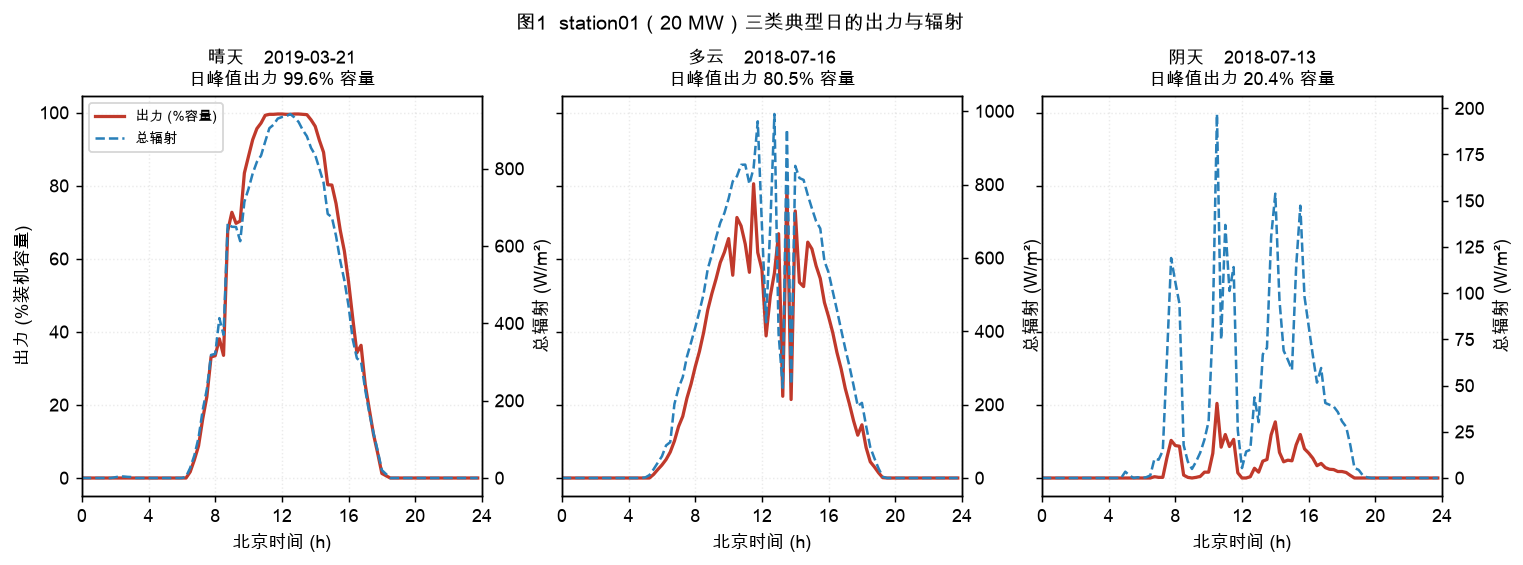
\includegraphics[width=0.95\textwidth]{fig1_typical_day}
\caption{station01 三类典型日的出力与辐射（已排除平顶异常日）}
\label{fig:typical}
\end{figure}

\begin{figure}[htbp]
\centering
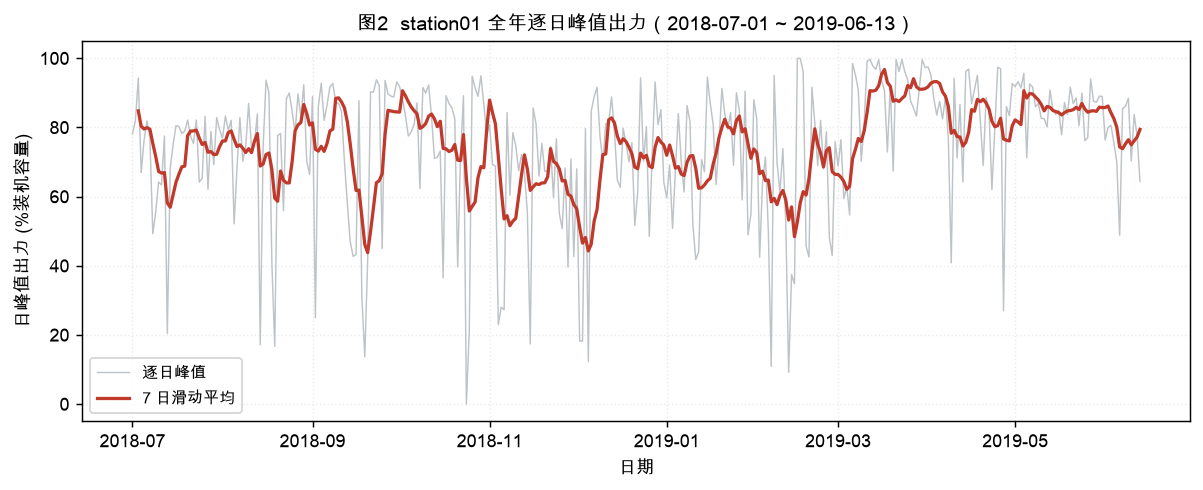
\includegraphics[width=0.95\textwidth]{fig2_daily_max}
\caption{station01 全年逐日峰值出力与 7 日滑动平均}
\label{fig:dailymax}
\end{figure}

\begin{figure}[htbp]
\centering
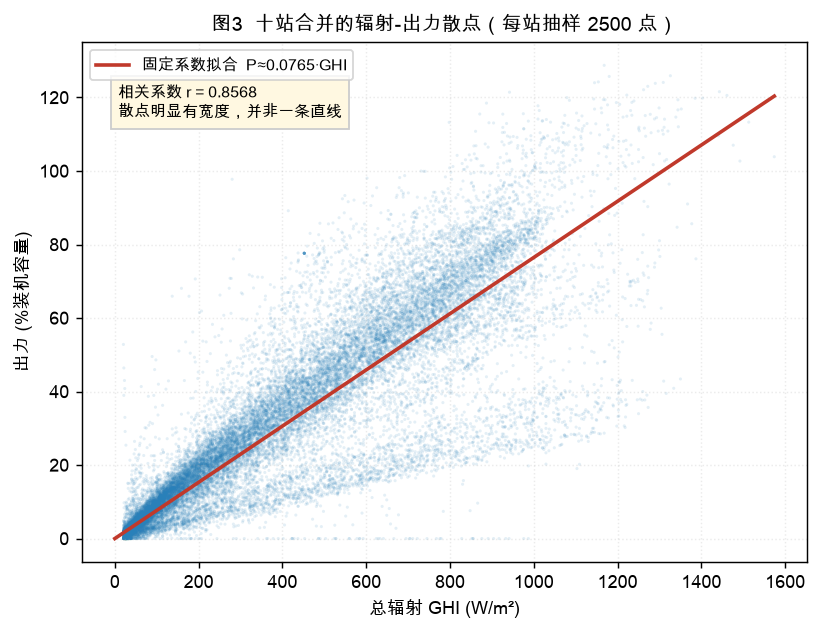
\includegraphics[width=0.8\textwidth]{fig3_scatter}
\caption{十站合并的辐射-出力散点图}
\label{fig:scatter}
\end{figure}

图 \ref{fig:typical} 给出晴、多云、阴三类典型日的曲线：晴天是光滑的钟形，日峰值出力达 99.6\% 容量；
多云日辐射被云层反复遮挡，出力随之剧烈起伏（峰值 80.5\%）；阴天辐射长期低平，出力仅 20.4\%。
图 \ref{fig:dailymax} 给出全年逐日峰值，可见冬季明显低于夏季，季节性强。
图 \ref{fig:scatter} 是辐射与出力的散点，相关系数 0.8568——注意散点并非一条细线而是有明显宽度，
这恰恰说明出力并不由辐射唯一决定，这正是设定丙中恒等映射项（上一刻功率）能派上用场的空间。

需要补充一点：图 \ref{fig:scatter} 的十站合并相关系数是 0.8568，
而后面逐站计算的相关平均有 0.9650，两者相差不小。
差的这一部分并不是随机噪声，而是各站装机容量与转换效率不同带来的系统性差异——
把不同规模的电站混在一起画散点，点自然就散开了。
这正是本文坚持按装机容量归一化、并且分站建模与评估的原因。

\begin{figure}[htbp]
\centering
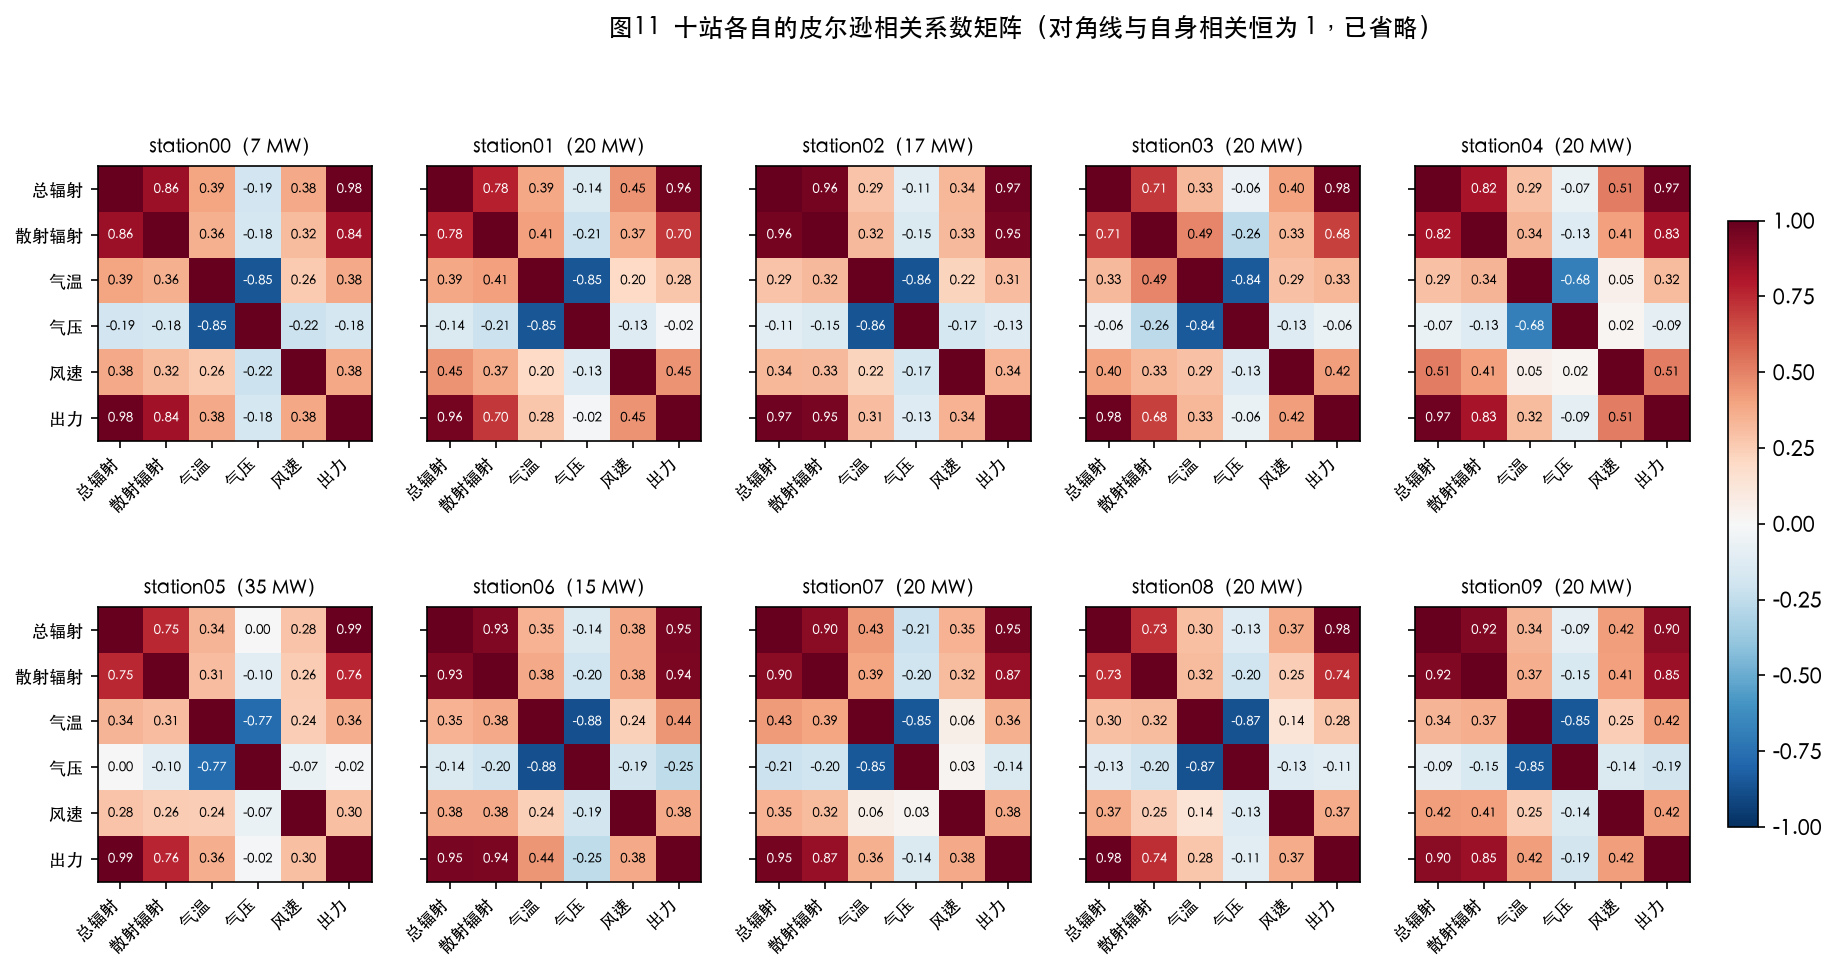
\includegraphics[width=\textwidth]{fig11_pearson_by_station}
\caption{十座电站各自的皮尔逊相关系数矩阵（对角线与自身相关恒为 1，已略去数值）}
\label{fig:pearson}
\end{figure}

\begin{figure}[htbp]
\centering
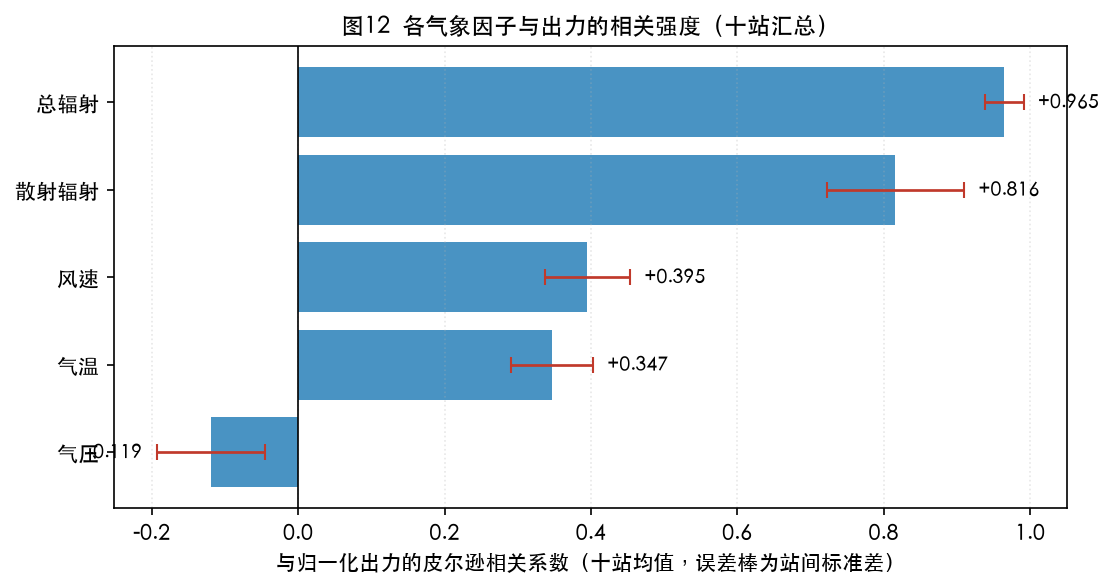
\includegraphics[width=0.86\textwidth]{fig12_corr_stability}
\caption{各气象因子与归一化出力的相关强度，误差棒为十站之间的标准差}
\label{fig:corrstab}
\end{figure}

第二组图看变量之间的相关结构。图 \ref{fig:pearson} 给出十个站各自的相关矩阵，
六个变量的排列次序在十个站上完全一致，说明这套数据的物理规律是稳定的，
不存在某座电站「性格特殊」到需要单独建模的程度。
图 \ref{fig:corrstab} 把「与出力的相关」单独抽出来，按十站均值排序并给出站间标准差，
结果见表 \ref{tab:pearson}。

\begin{table}[htbp]
\centering
\small
\caption{各气象因子与归一化出力的皮尔逊相关系数（十站统计）}
\label{tab:pearson}
\begin{tabular}{lcccc}
\toprule
变量 & 十站均值 & 站间标准差 & 最小 & 最大 \\
\midrule
总辐射   & 0.9650 & 0.0260 & 0.9018 & 0.9908 \\
散射辐射 & 0.8160 & 0.0937 & 0.6807 & 0.9519 \\
风速     & 0.3951 & 0.0582 & 0.2976 & 0.5114 \\
气温     & 0.3468 & 0.0559 & 0.2759 & 0.4395 \\
气压     & $-0.1189$ & 0.0741 & $-0.2509$ & $-0.0191$ \\
\bottomrule
\end{tabular}
\end{table}

总辐射以 0.9650 的相关度居首，且站间标准差只有 0.0260，
说明它是十站通用的、最可靠的预测依据；散射辐射次之（0.8160），但站间波动明显变大。
风速与气温的相关都只有 0.4 上下；气压甚至接近 0。

\begin{figure}[htbp]
\centering
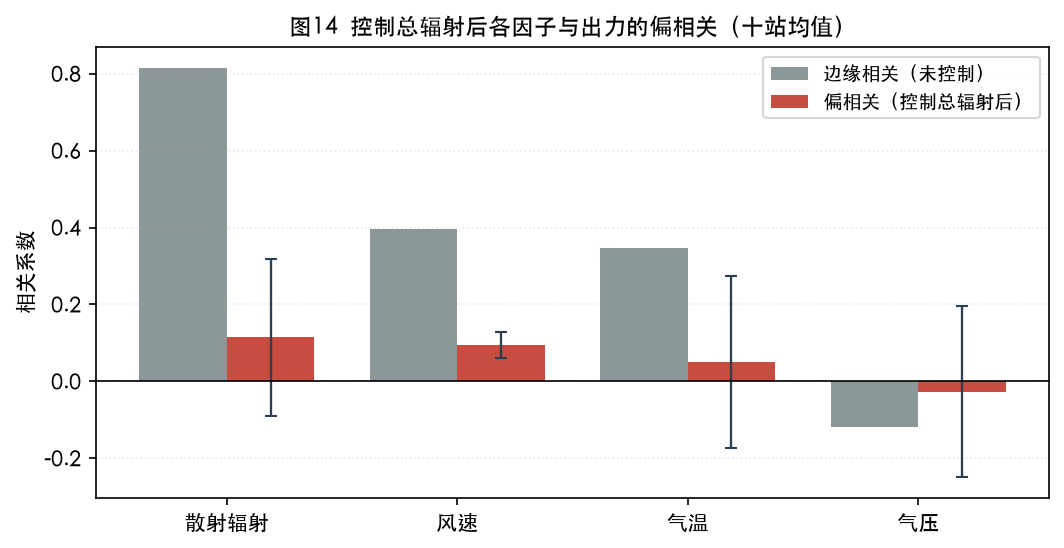
\includegraphics[width=0.86\textwidth]{fig14_partial_corr}
\caption{控制总辐射后各因子与出力的偏相关（十站均值，误差棒为站间标准差）}
\label{fig:partial}
\end{figure}

这里有一个必须澄清的疑点。按光伏物理常识，组件温度升高会使开路电压下降、效率降低，
因此气温与出力之间应当呈\textbf{负}相关；但表 \ref{tab:pearson} 显示它是 $+0.3468$，符号相反。
这是不是说明数据有问题？并不是。原因是气温与总辐射高度共线——夏天既热又晒，
于是「热」和「发电多」在统计上被绑在了一起，形成典型的混淆相关。

为验证这一点，本文计算了控制总辐射之后的一阶偏相关
\[
r(xy\mid z)=\frac{r_{xy}-r_{xz}r_{yz}}{\sqrt{(1-r_{xz}^2)(1-r_{yz}^2)}} ,
\]
结果见图 \ref{fig:partial}：气温与出力的相关从 $+0.3468$ 掉到 $+0.0504$，
几乎归零，且站间标准差高达 0.2231——也就是说残余关联在十个站上连符号都不一致。
风速也从 $+0.3951$ 降到 $+0.0940$。

这个结果有两层含义。其一，气温对光伏效率的影响是真实存在的物理效应，
但在本数据中被与辐射的共线关系掩盖了，模型分不开二者，
这正好解释了 \ref{sec:ablation} 节消融实验里「删掉温度特征模型几乎不变」的现象，
也提醒我们不能把该结果误读成「温度对光伏没有影响」。
其二，相关矩阵只能说明变量长得像不像，不能说明谁重要；
真正的贡献要由后面特征重要性与消融实验来回答。

\begin{figure}[htbp]
\centering
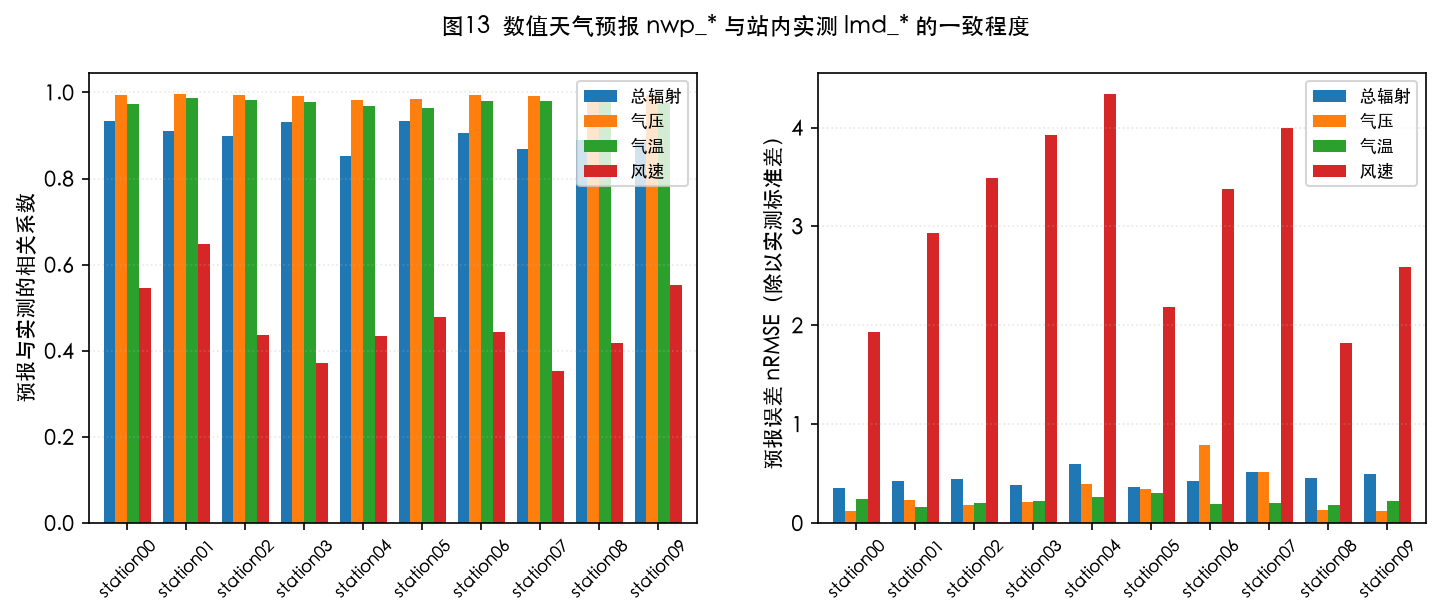
\includegraphics[width=\textwidth]{fig13_nwp_vs_lmd}
\caption{数值预报 $nwp\_*$ 与站内实测 $lmd\_*$ 的一致程度（十座电站）}
\label{fig:nwp}
\end{figure}

第三组图检验预报值是否靠得住，因为它直接决定设定甲$'$ 能做到多好。
图 \ref{fig:nwp} 给出同名变量的预报值与实测值的相关与归一化误差，
十站平均见表 \ref{tab:nwp}。

\begin{table}[htbp]
\centering
\small
\caption{预报值与实测值的一致程度（十站平均，nRMSE 为误差除以实测量的标准差）}
\label{tab:nwp}
\begin{tabular}{lcc}
\toprule
变量 & 相关系数 & nRMSE \\
\midrule
总辐射 & 0.9010 & 0.4455 \\
气温   & 0.9773 & 0.2195 \\
气压   & 0.9917 & 0.3038 \\
风速   & 0.4682 & 3.0611 \\
\bottomrule
\end{tabular}
\end{table}

气温与气压的预报相当准（相关 0.98 以上），但\textbf{总辐射的预报误差达到实测波动幅度的 44.55\%}，
风速预报更是几乎不可用（相关仅 0.4682）。
总辐射恰恰是预测出力最关键的那一个变量，它的预报误差会原样传导到功率预测上，
这解释了为什么设定甲$'$ 的误差（4.8725）几乎是设定甲（2.4738）的两倍。

% ------------------------------------------------------------

\subsection{总体预测性能}
\label{sec:overall}

\begin{table}[htbp]
\centering
\small
\caption{四个设定下的十站平均预测误差（MAE 与 RMSE 单位为 \%装机容量）}
\label{tab:metrics}
\begin{tabular}{llccc}
\toprule
设定 & 方法 & MAE & RMSE & 相对基线改善 \\
\midrule
\multirow{6}{*}{甲$'$ 预报气象}
 & 随机森林        & \textbf{4.8725} & \textbf{9.6291} & \textbf{13.88\%} \\
 & LightGBM        & 4.9060 & 9.2251 & 13.28\% \\
 & XGBoost         & 5.2421 & 9.7543 & 7.34\%  \\
 & GBDT            & 5.3871 & 9.6372 & 4.78\%  \\
 & 朴素基线: 固定系数 & 5.6575 & 10.6433 & ---    \\
 & 线性回归        & 6.3862 & 10.1306 & $-12.88\%$ \\
\midrule
\multirow{6}{*}{甲 实测气象}
 & LightGBM        & \textbf{2.4738} & \textbf{5.3336} & \textbf{18.58\%} \\
 & 随机森林        & 2.5202 & 5.6232 & 17.05\% \\
 & XGBoost         & 2.7123 & 5.7719 & 10.73\% \\
 & 朴素基线: 固定系数 & 3.0383 & 6.2068 & ---    \\
 & GBDT            & 3.0652 & 5.9454 & $-0.89\%$ \\
 & 线性回归        & 3.6613 & 6.2300 & $-20.50\%$ \\
\midrule
\multirow{6}{*}{乙 纯历史}
 & LightGBM        & \textbf{2.2821} & \textbf{5.2633} & \textbf{11.57\%} \\
 & 随机森林        & 2.4364 & 5.5432 & 5.60\%  \\
 & 朴素基线: Persistence & 2.5808 & 5.6427 & ---  \\
 & 线性回归        & 2.5324 & 5.2839 & 1.88\%  \\
 & GBDT            & 2.5467 & 5.5861 & 1.32\%  \\
 & XGBoost         & 2.6552 & 5.8380 & $-2.88\%$ \\
\midrule
\multirow{6}{*}{丙 实测气象$+$历史}
 & 线性回归        & \textbf{1.4942} & \textbf{3.1507} & \textbf{41.74\%} \\
 & LightGBM        & 1.6376 & 3.8300 & 36.15\% \\
 & 随机森林        & 1.6689 & 4.0761 & 34.93\% \\
 & XGBoost         & 1.7520 & 4.0221 & 31.69\% \\
 & GBDT            & 1.8384 & 4.0114 & 28.32\% \\
 & 朴素基线: Persistence & 2.5648 & 5.6214 & ---  \\
\bottomrule
\end{tabular}
\end{table}

表 \ref{tab:metrics} 给出四个设定下的全部结果。逐层看下来，有三点值得说。

第一，信息越全，误差越小，且增益主要来自「同时刻气象」而非「更多模型」。
设定乙只有历史观测，最好的 LightGBM 为 2.2821；加入同时刻实测气象（设定丙）后降到 1.4942，
误差减少约三分之一。把同时刻实测气象换成数值天气预报（设定甲$'$），
最好的随机森林为 4.8725，几乎是设定甲（2.4738）的两倍——预报误差本身就值这么多。
这个对照说明：对这类超短期预测，接入一条实时气象实测，比换一个更复杂的模型更划算。

第二，在条件最苛刻的设定乙里，机器学习确实管用，但增益有限且不稳。
LightGBM 把 MAE 从 Persistence 的 2.5808 降到 2.2821，降幅 11.57\%；
随机森林降 5.60\%；而 XGBoost 反而比基线差 2.88\%。
差距之所以不大，原因在特征重要性里——设定乙中「上一刻功率」一项就占了 96\% 的重要性（见 \ref{sec:importance} 节），
模型能做的只是对这条强特征做小幅修正。

第三，也是本文最意外的一点：在设定丙中，表现最好的是线性回归，而不是任何树模型。
它比第二名的 LightGBM 低 8.8\%，比 Persistence 低 41.74\%，且 $R^2$ 达 0.9849，是全场唯一超过 0.98 的。
这个结果反直觉，需要专门解释，见下一小节。


% ------------------------------------------------------------
\subsection{单站深度模型对照：复杂模型是否一定更好}
\label{sec:lstmsingle}

前面几节的比较都停留在「朴素基线 vs 树模型 vs 线性回归」这一层。
本节把 LSTM 也放进同一条件，回答研究问题一：模型越复杂，预测一定越准吗？

实验条件与 \ref{sec:overall} 节完全一致：同一份数据、同一条前 70\%/后 30\% 的时间切分、
同一套信息可得性约束。LSTM 取两层、隐藏单元 64、回看窗口 12 步（3 小时）、
Adam 学习率 $10^{-3}$、固定训练 30 轮，未做早停与超参搜索；树模型统一 100 棵树、学习率 0.1。
两者唯一的差别是输入的组织方式：树模型看到的是若干个人工构造的滞后特征
（$GHI$ 滞后 1/2/3/6/12 步、上一刻功率等），LSTM 看到的是过去 3 小时逐点的多变量序列，
二者覆盖的时间跨度相当，信息量可比，因此这个对照是公平的。
需要说明的是，跨时间的断点窗口已被剔除，避免把几天前的同一时刻当成连续历史。

\begin{table}[htbp]
\centering
\small
\caption{单站内六类方法的十站平均 MAE（\%装机容量）与单站平均训练耗时（秒）}
\label{tab:lstmsingle}
\begin{tabular}{llcc}
\toprule
设定 & 方法 & MAE & 训练耗时(s) \\
\midrule
\multirow{6}{*}{甲 实测气象}
 & LightGBM        & \textbf{2.4738} & 0.47 \\
 & 随机森林        & 2.5202 & 1.76 \\
 & XGBoost         & 2.7123 & 0.17 \\
 & 朴素基线：固定系数 & 3.0383  & ---  \\
 & LSTM            & 3.1467  & 9.63 \\
 & 线性回归        & 3.6613  & 0.00 \\
\midrule
\multirow{6}{*}{甲$'$ 预报气象}
 & 随机森林        & \textbf{4.8725} & 2.60 \\
 & LightGBM        & 4.9060 & 0.48 \\
 & XGBoost         & 5.2421 & 0.20 \\
 & 朴素基线：固定系数 & 5.6575  & ---  \\
 & LSTM            & 5.9380  & 9.63 \\
 & 线性回归        & 6.3862  & 0.00 \\
\midrule
\multirow{6}{*}{乙 纯历史}
 & LightGBM        & \textbf{2.2821} & 0.49 \\
 & 随机森林        & 2.4364 & 2.59 \\
 & 线性回归        & 2.5324  & 0.00 \\
 & 朴素基线：Persistence & 2.5808 & --- \\
 & XGBoost         & 2.6552 & 0.19 \\
 & LSTM            & 4.1694  & 9.63 \\
\midrule
\multirow{6}{*}{丙 气象+历史}
 & 线性回归        & \textbf{1.4942} & 0.00 \\
 & LightGBM        & 1.6376 & 0.42 \\
 & 随机森林        & 1.6689 & 2.36 \\
 & XGBoost         & 1.7520 & 0.17 \\
 & 朴素基线：Persistence & 2.5648 & --- \\
 & LSTM            & 3.1624  & 9.63 \\
\bottomrule
\end{tabular}
\end{table}

\begin{figure}[htbp]
\centering
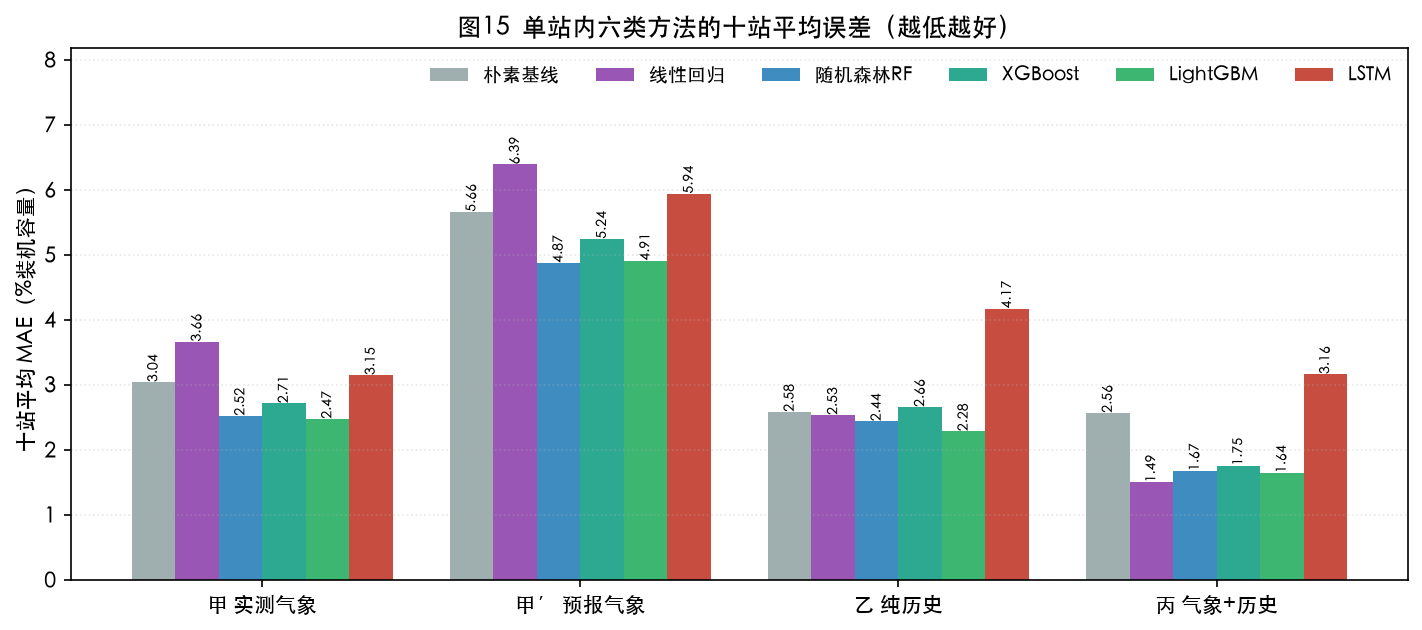
\includegraphics[width=\textwidth]{fig15_single_station_compare}
\caption{单站内六类方法在四个设定下的十站平均误差}
\label{fig:singlecompare}
\end{figure}

结果相当干脆：LSTM 在四个设定上\textbf{全部落后}，见表 \ref{tab:lstmsingle} 与图 \ref{fig:singlecompare}。
最好情况下（设定甲$'$）它比最优树模型差 21.9\%，最差情况下（设定丙）差 111.6\%；
在设定乙里它甚至输给了完全不需要训练的 Persistence 基线 61.6\%。
也就是说，本任务上「更复杂的模型」带来的不是精度提升，而是明确的负收益。

为什么会这样？本文给出三点解释。

第一，这个任务几乎不需要「记忆」。光伏出力与同时刻辐射之间是近似瞬时的物理映射，
决定当前出力的是「现在晒不晒」，而不是「三小时前晒不晒」。
LSTM 的核心能力是捕捉长程时间依赖，而这项能力在本任务上恰好用不上——
真正需要的信息（当前辐射、上一刻功率）在输入里已经直接给出了，
让模型再去从序列里「回忆」一遍，反而增加了拟合难度。

第二，数据量与模型容量不匹配。每站约 1\,$\sim$\,3.3 万条记录，
对需要大量样本才能估稳参数的神经网络来说偏少；树模型在小样本上天然更稳健。

第三，序列里混进了大量夜间段。十个站的夜间样本平均占 49.07\%，这些时段出力恒为 0，
与白天的物理规律完全不同。LSTM 必须用同一套权重同时学会「夜间恒零」和「白天跟随辐射」两种模式；
而树模型只要看一眼辐射值就能把两者彻底分开。这是结构上的劣势，不是调参能弥补的。

还有一点值得单独指出：训练代价相差悬殊。表 \ref{tab:lstmsingle} 最后一列显示，
线性回归只需 0.003 秒、LightGBM 约 0.47 秒，而 LSTM 需要约 9.6 秒，
是线性回归的三千余倍，精度却更差；若把调参成本也计入，差距只会更大。
这对工程选型是一个很实际的提醒：在这类表格型回归任务上，
先把基线模型和树模型做到位，往往比直接上深度模型划算得多。

需要说明的是，这并不意味着深度模型在光伏预测中没有价值——
它只是说明在「单站、中等数据量、以同时刻物理量为主」这一特定条件下不够划算。
下一节会看到，当任务换成跨站迁移时，LSTM 的表现规律与树模型并不相同。

% ------------------------------------------------------------

\subsection{树模型为什么学不好「上一刻功率」}
\label{sec:identity}

上一小节留下的问题是：为什么线性回归能在设定丙中胜出。本文的假说是，
Persistence 本质上是一个硬编码的恒等映射 $P(t)=1.0\times P(t-1)$；
线性回归能学到接近 1 的系数从而复现它，而树模型只能输出叶节点内训练样本的均值，
天生做不到「输出等于输入」，于是把高值压低、低值抬高。

为验证这个假说，本文做了一个极简对照：每站只用「上一刻功率」一个特征，
分别用硬编码的 Persistence、线性回归与随机森林预测，结果见表 \ref{tab:identity}。

\begin{table}[htbp]
\centering
\caption{恒等映射检验：每站只用「上一刻功率」一个特征（十站平均，MAE 单位 \%装机容量）}
\label{tab:identity}
{\small
\begin{tabular}{lccp{4.6cm}}
\toprule
预测方式 & 十站平均 MAE & 相对 Persistence & 说明 \\
\midrule
Persistence（硬编码系数 1.0）         & \textbf{2.5648} & ---      & 直接令 $P(t)=P(t-1)$ \\
线性回归（学到系数 $k$）              & 2.7136 & $-5.80\%$ & 系数 $k$ 落在 $0.9744\sim0.9874$，平均 0.9788 \\
随机森林（200 棵，分段常数）          & 3.1521 & $-22.90\%$ & 无法表达恒等映射 \\
\bottomrule
\end{tabular}}
\end{table}

结果支持该假说。随机森林单独用这一个特征时，比直接把该特征当预测值差了 22.90\%；
线性回归学到的系数在十站上都接近 1（0.9744$\sim$0.9874），比随机森林好，但仍略逊于硬编码的 1.0，
因为最小二乘为压低整体误差而把系数往均值方向拉了一点。

这一机制同时解释了另外两个现象。其一，设定丙中线性回归胜出：
它既能写出 $P\approx0.98\times P(t-1)$ 的恒等映射，又能用气象项做线性修正，
而树模型在分段平均时会破坏恒等关系。其二，\ref{sec:weather} 节将展示，
在辐射平稳的时段随机森林反而大幅输给 Persistence——正因为那些时刻几乎就是恒等映射。

需要说明的是，这不代表「越简单的模型越好」。在设定甲$'$（预报气象）中，
线性回归是全表最差的（$-12.88\%$），说明当输入与目标的关系明显非线性时，线性模型就会失效。
真正稳妥的说法是：在含强自回归项的设定里，线性基线与树模型应当并列比较，不能想当然地只上树模型。

\subsection{误差的天气分布（拓展一）}
\label{sec:weather}

\begin{figure}[htbp]
\centering
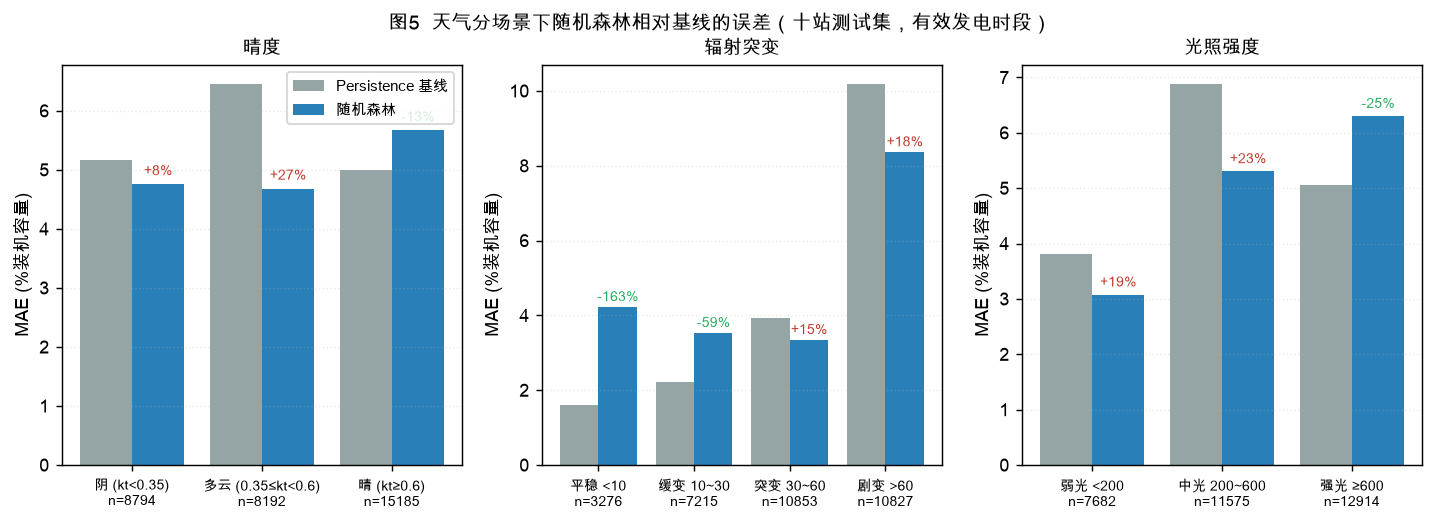
\includegraphics[width=0.95\textwidth]{fig5_weather_scenarios}
\caption{不同天气场景下随机森林相对 Persistence 基线的误差}
\label{fig:weather}
\end{figure}

把十站测试集合并，按晴度（晴空指数 $kt$）、辐射突变强度（$|\Delta \mathrm{GHI}|$）、
光照强度（GHI）三个维度分组，结果见图 \ref{fig:weather}。为排除干扰，
此处只统计有效发电时段（实测总辐射大于 50\,W/m$^2$），并在计算晴空指数前先限定太阳高度角——
否则日出日落附近大气路径极长、$kt$ 天然偏低，会把「阴天」这一档撑得特别大，那不是云造成的。

中栏（辐射突变强度）的结论最清晰：模型增益几乎全部集中在辐射有变化的时候。
突变 30$\sim$60\,W/m$^2$ 一组（10853 个样本）降幅 14.54\%，剧变超过 60\,W/m$^2$ 一组（10827 个样本）降幅 17.90\%；
而辐射平稳（$<$10\,W/m$^2$，3276 个样本）时，随机森林 MAE 为 4.2285，反而比 Persistence 的 1.6077 差了 163\%。
这正是上一小节所说的恒等映射问题：辐射平稳意味着功率也平稳，此时 Persistence 已接近最优，
模型再去拟合只会引入额外波动。

左栏（晴度）表现为：多云（$0.35\le kt<0.6$，8192 样本）降幅最大，达 27.50\%；
阴天（$kt<0.35$，8794 样本）降幅 7.74\%；晴天（$kt\ge0.6$，15185 样本）反而为 $-13.42\%$。
晴天的负值同样符合上述逻辑——万里无云时辐射曲线光滑，Persistence 本身就非常准。

右栏（光照强度）中，中光（200$\sim$600\,W/m$^2$，11575 样本）降幅 23.03\%、弱光 19.27\%，
而强光（$\ge$600，12914 样本）为 $-24.72\%$。强光时段多为晴空，与左栏晴天一致。

综合三栏可以给出一条工程上可用的判据：\textbf{Persistence 在平稳晴好天气下是天然强基线，
不应被直接忽略；模型的价值集中在云层扰动导致辐射起伏的时段。}
实际部署时宜按辐射突变强度切换预测策略，而不是全天只跑一个模型。

\subsection{特征重要性（拓展二）}
\label{sec:importance}

\begin{figure}[htbp]
\centering
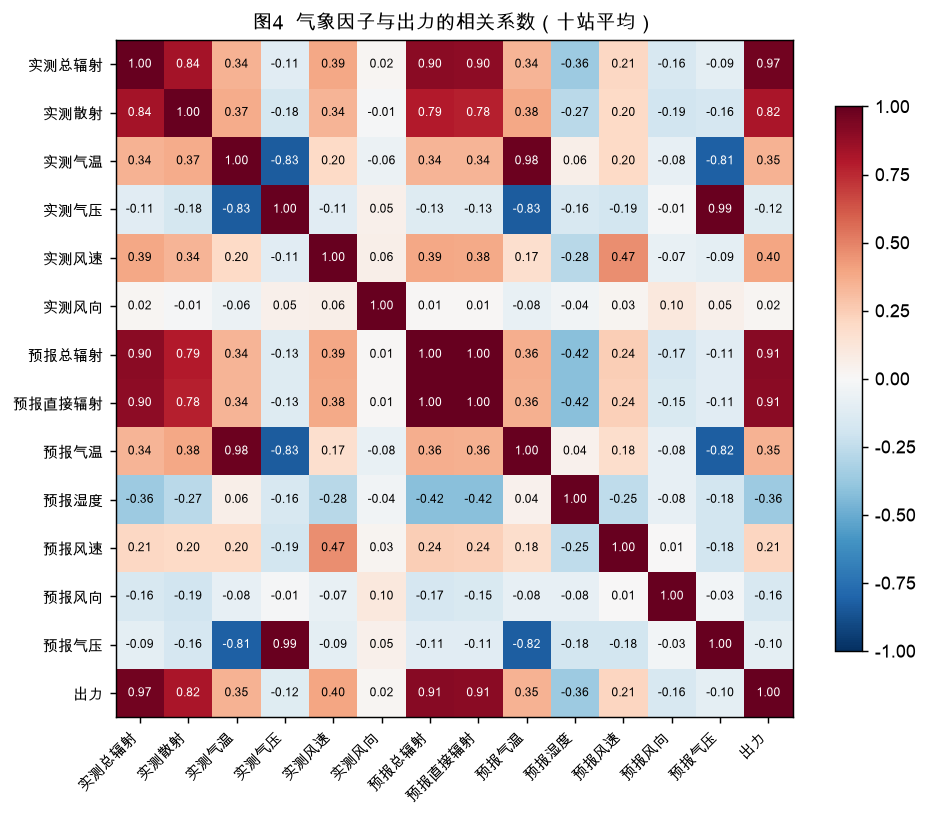
\includegraphics[width=0.78\textwidth]{fig4_corr}
\caption{气象因子与出力的相关系数（十站平均）}
\label{fig:corr}
\end{figure}

图 \ref{fig:corr} 先给出相关分析的全局印象：站内实测总辐射与出力的相关系数最高，
预报总辐射与预报直接辐射次之，气温、气压、风速、风向等与出力的相关性则明显偏低，
且实测与预报两组变量之间自身高度相关。这预示了后面消融实验的结果——
辐射类之外的气象因子能提供的信息有限。

\begin{figure}[htbp]
\centering
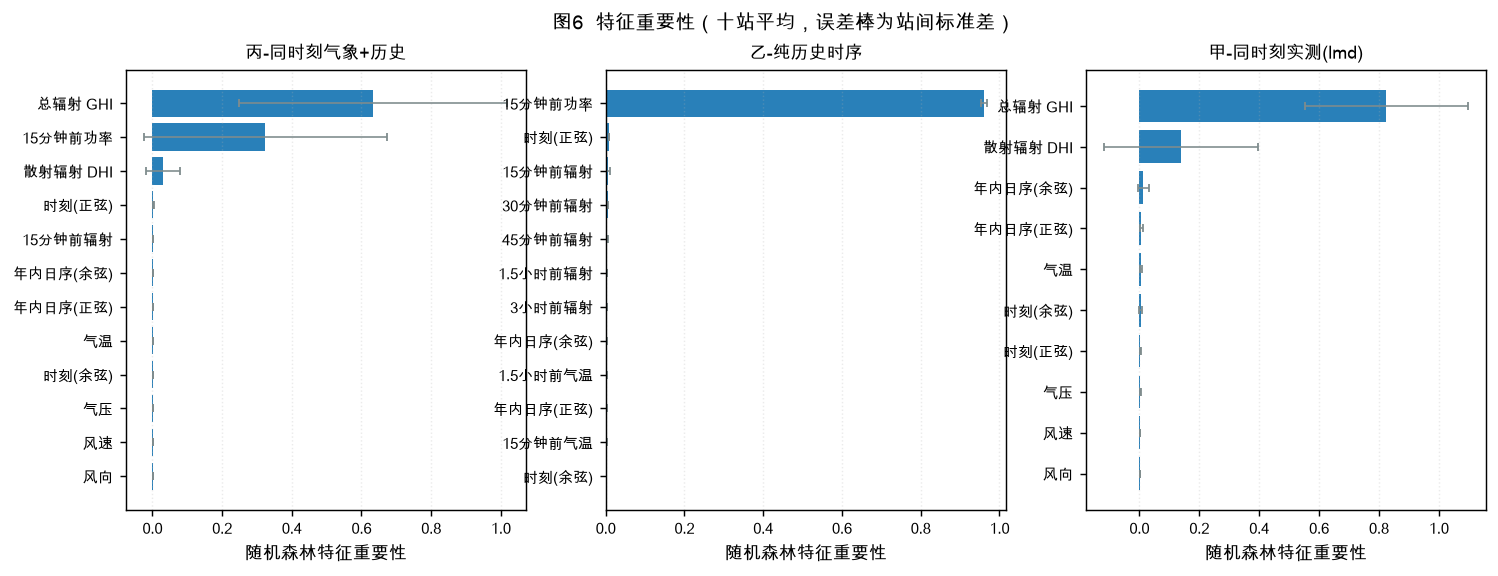
\includegraphics[width=0.95\textwidth]{fig6_feature_importance}
\caption{三个设定下随机森林特征重要性的十站平均排序（误差棒为站间标准差）}
\label{fig:importance}
\end{figure}

图 \ref{fig:importance} 给出三个设定的特征重要性排序，取十站平均（单站排序有偶然性，十站平均才稳），
误差棒表示站间标准差。

设定乙中，上一刻功率 $P$\_lag1 的重要性高达 0.961，站间标准差仅 0.007，
其余十一个特征合计不足 0.04。这直观说明为什么设定乙的提升有限——信息几乎全在一条特征里。
滞后辐射 GHI\_lag2 至 lag12 的重要性虽小却稳定非零，它们的作用是当辐射突变、上一刻功率失效时提供补充。

设定丙中格局变成 GHI 0.634 与 $P$\_lag1 0.324 两强并立，两者合计约 96\%，
散射辐射贡献 0.030，其余特征均在 0.003 以下。
这个结构正好对应 \ref{sec:overall} 节：既要有「同时刻辐射」定位当前天气，也要有「上一刻功率」提供恒等映射的锚点。

设定甲（实测气象）中总辐射 0.824、散射辐射 0.139 合计 96.3\%，气象因子里只有辐射类起作用。
设定甲$'$（预报气象）则不同：预报总辐射 0.384 与预报直接辐射 0.360 相加也只有 0.744，
时刻余弦编码占到 0.119，气压、湿度、风向等也各有贡献（合计约 0.106）。
原因是预报辐射本身带有误差，模型无法仅靠它定出出力，只好借助时刻与季节信息来补偿——
这也从侧面印证了 \ref{sec:overall} 节「预报误差直接转化为精度损失」的结论。

\subsection{特征消融（拓展二补充）}
\label{sec:ablation}

\begin{table}[htbp]
\centering
\small
\caption{特征消融：整组删掉某类特征后的十站平均 MAE（随机森林，单位 \%装机容量；「相对完整」按十站平均 MAE 计算）}
\label{tab:ablation}
\begin{tabular}{llccc}
\toprule
设定 & 特征集 & 特征数 & MAE & 相对完整 \\
\midrule
\multirow{3}{*}{丙 实测气象$+$历史}
 & 完整                & 12 & \textbf{1.6689} & ---     \\
 & 删全部同时刻气象     & 6  & 2.6952 & $+61.49\%$ \\
 & 只留上一刻功率       & 5  & 2.7131 & $+62.56\%$ \\
\midrule
\multirow{4}{*}{乙 纯历史}
 & 完整                & 12 & 2.4364 & ---     \\
 & 删气温滞后           & 10 & 2.4237 & $-0.52\%$ \\
 & 删时刻编码           & 8  & 2.4385 & $+0.09\%$ \\
 & 只留上一刻功率       & 5  & 2.7131 & $+11.36\%$ \\
\midrule
\multirow{3}{*}{甲 实测气象}
 & 完整                & 10 & 2.5202 & ---     \\
 & 删气温              & 9  & 2.5250 & $+0.19\%$ \\
 & 删气温$+$气压$+$风速 & 7  & 2.4837 & $-1.45\%$ \\
\bottomrule
\end{tabular}
\end{table}

\begin{figure}[htbp]
\centering
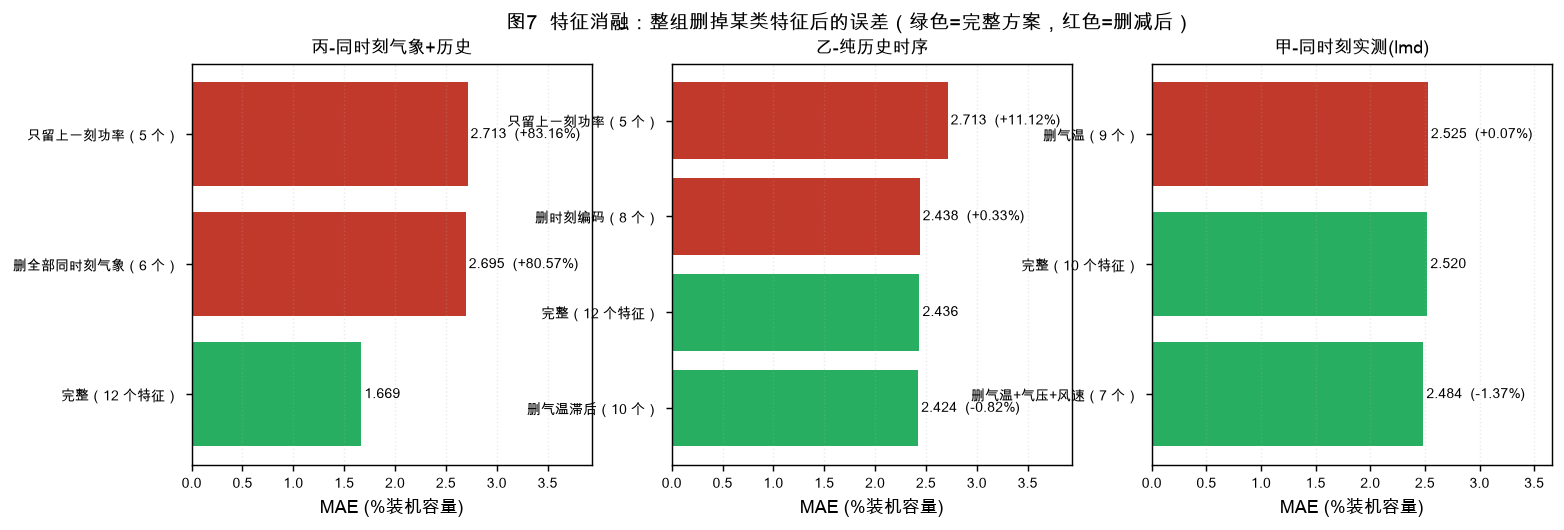
\includegraphics[width=0.95\textwidth]{fig7_ablation}
\caption{特征消融结果（绿色为完整方案，红色为删减后）}
\label{fig:ablation}
\end{figure}

表 \ref{tab:ablation} 给出消融结果，图 \ref{fig:ablation} 为对应柱状图。四组结论如下。

\textbf{（1）同时刻气象的贡献是决定性的。}设定丙中，把 6 个同时刻气象变量整组删掉，
MAE 由 1.6689 恶化到 2.6952，增加 61.49\%；删到只剩上一刻功率时恶化 62.56\%。
这说明即便已经有了自回归项，同时刻气象仍携带大量独立信息，两者不可互相替代。

\textbf{（2）次要气象因子（气温、气压、风速）几乎没有独立贡献。}
设定甲中删掉气温，MAE 只变化 0.19\%；连气温、气压、风速一起删（10 个特征减到 7 个），
MAE 反而略降 1.45\%。这提示在辐射类特征已在场的情况下，这些气象量提供的信息已被吸收。

\textbf{（3）时间特征工程（时刻正余弦编码）的收益很小。}
设定乙中删掉 4 个时刻编码，MAE 仅从 2.4364 变为 2.4385，恶化 0.09\%。
这与预期不同——一般认为时刻编码能帮助模型识别日内规律。可能的原因是：
滞后辐射与滞后功率本身已经隐含了时刻信息（日出前后辐射自然低），时刻编码提供的增量因此有限。
本文如实记录这一结果，不因为它「看起来应该有用」就把它写成有效。

\textbf{（4）气温滞后删掉后误差不升反降（$-0.52\%$）。}
这与第（2）条一致，同样说明温度相关特征在本数据上不带来可测增益。

需要强调一点：以上消融结果只能说明「在本数据、本特征组合下，这些变量不带来可测增益」，
不能推广成「温度对光伏出力没有物理影响」。光伏组件的温度效应确实存在（约 $-0.3 \sim -0.4\ \%/^{\circ}\mathrm{C}$），
只是它在本数据里与辐射高度共线，被辐射效应吸收，模型无法把两者分开。

\subsection{跨站迁移检验（拓展三）}
\label{sec:transfer}

前文所有结论都来自同一条流水线，换一座电站是否仍然成立，尚未检验。本节回答这个问题。

\begin{table}[htbp]
\centering
\caption{留一站交叉验证的四方案对比（全天口径，MAE 与 RMSE 单位为 \%装机容量）；表内「相对 A 的改善」为逐站算出后再取平均，与 MAE 列的十站平均口径略有差异。}
\label{tab:transfer}
\begin{tabular}{lccrc}
\toprule
方案 & MAE & RMSE & 相对 A 的改善 & 优于 A 的站数 \\
\midrule
A 从零训练      & 2.744 & 5.731  & ---         & ---   \\
B 预训练 + 微调 & 2.584 & 5.455  & $-0.36\%$   & 6/10  \\
C 零样本迁移    & 4.657 & 8.614  & $-68.11\%$  & 3/10  \\
D 多站联合训练  & \textbf{2.315} & \textbf{5.030} & \textbf{+14.61\%} & \textbf{8/10} \\
\bottomrule
\end{tabular}
\end{table}

\begin{figure}[htbp]
\centering
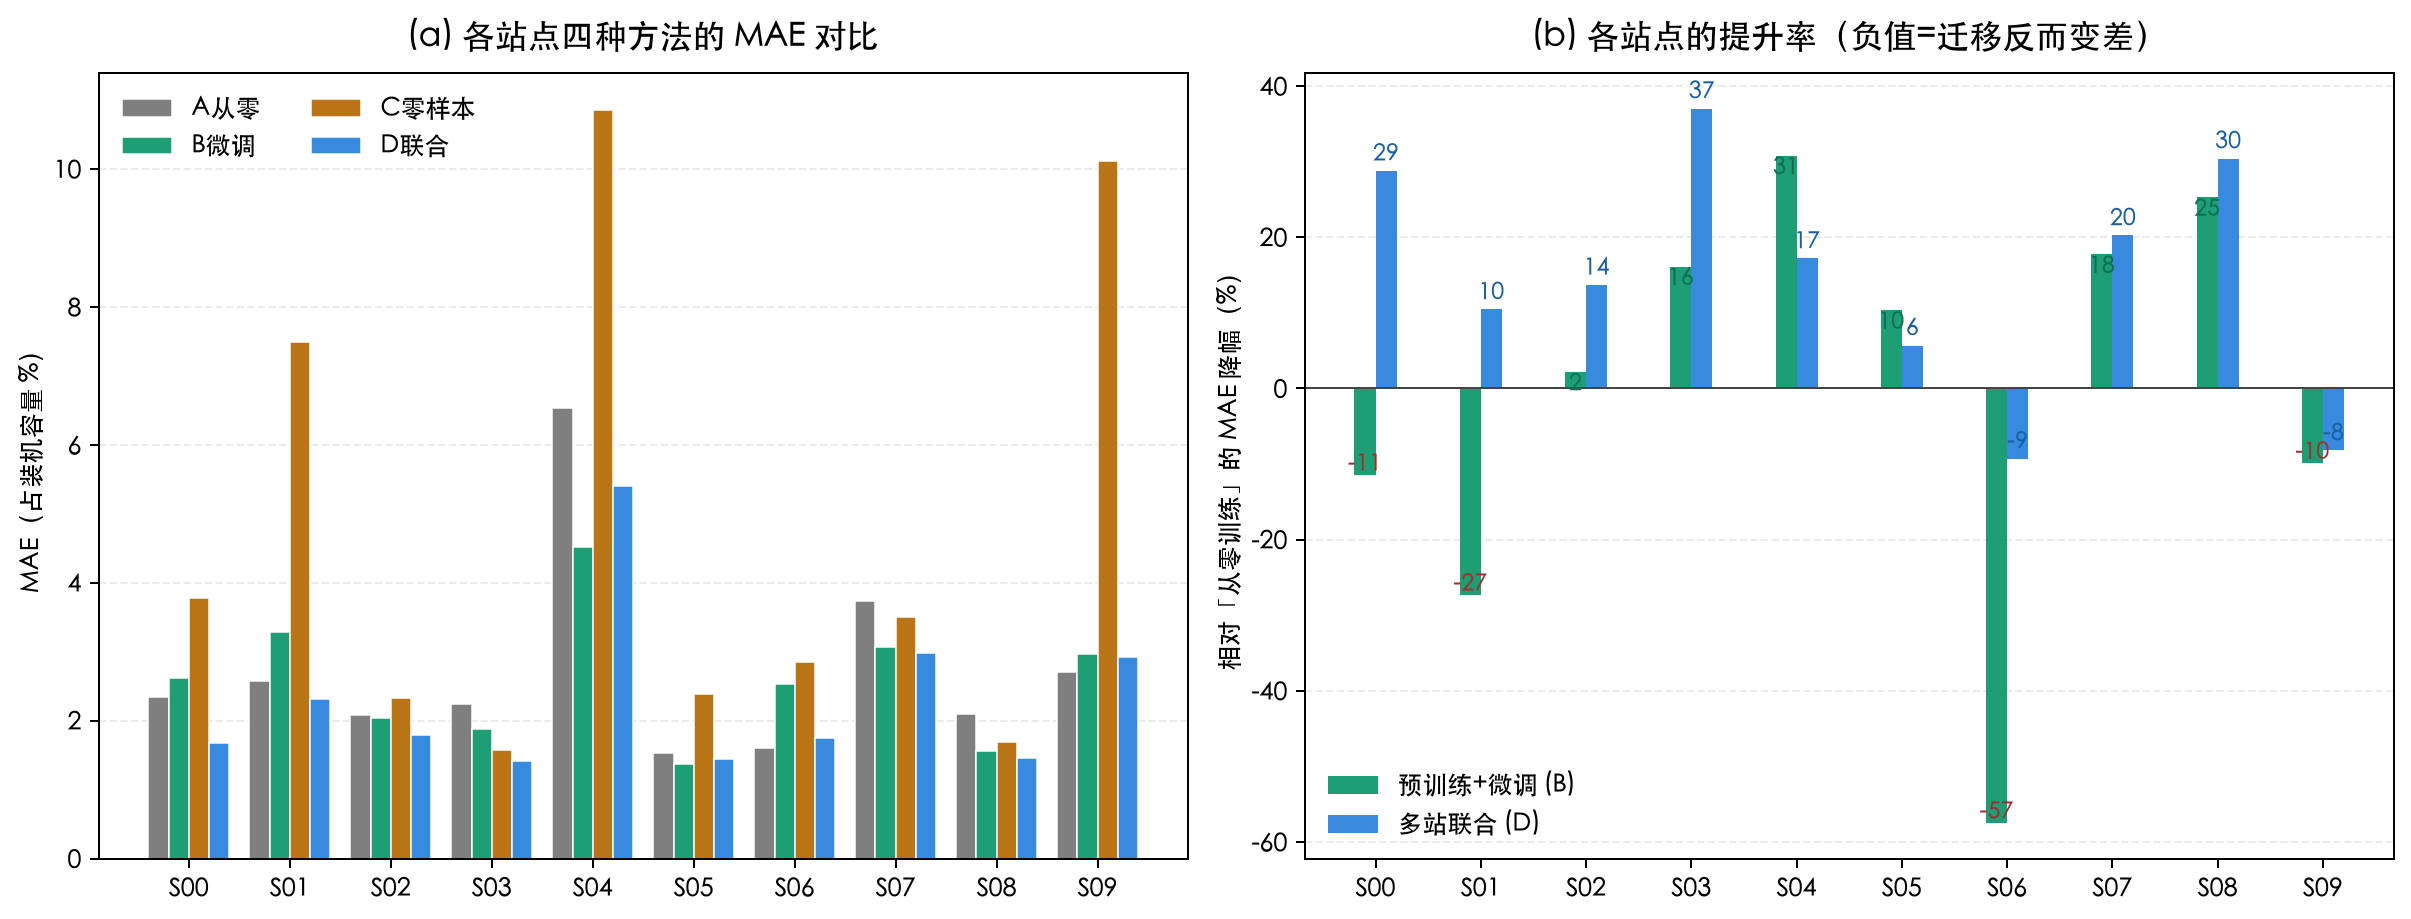
\includegraphics[width=0.95\textwidth]{fig8_transfer_loso}
\caption{留一站交叉验证结果：（a）各站 MAE 对比；（b）相对从零训练的改善幅度}
\label{fig:transfer}
\end{figure}

表 \ref{tab:transfer} 给出十站平均结果，排序为 $D>B>A>C$。
多站联合训练平均把误差压低 14.61\%，八个站改善；
预训练后微调则几乎没有作用，平均仅 $-0.36\%$，只有六个站改善。
两者的差别在于：微调是在别人已经成型的 500 棵树上再追加 200 棵，
老树始终参与预测、改不掉，目标站的数据只能影响新加的那部分树；
联合训练从一开始就把目标站数据混进去，样本权重又把目标站样本放大 5 倍以抵消数量劣势，
模型没有先入为主的包袱，因此更直接有效。

需要说明本节的输入口径。这里用的是站内实测气象 $lmd\_*$，
与 \ref{sec:overall} 节的设定甲一致，以便两组结果可以横向比较。
在预备阶段本文也曾用预报气象 $nwp\_*$ 跑过同一套实验，当时得到的提升幅度明显更大
（B 17.83\%、D 24.77\%），但那份结果既未做时区修正、口径也与主线不符，已作废。
两套结果的差别本身很有信息量：当本站已有高信息量的实测气象时，单站模型已经足够强，
跨站迁移能带来的边际收益就小；反过来，如果输入只能依赖误差较大的预报值，
迁移的价值就会凸显。也就是说，迁移值不值得做，取决于本站信息条件的贫富。

夜间出力恒为 0，容易预测，会把全天口径的 MAE 拉低。本文因此同时统计只含辐射大于 0 的白天口径：
A 为 4.532、B 为 4.343（$-1.15\%$）、C 为 8.045（$-71.32\%$）、D 为 3.886（$+13.29\%$），
排序与全天口径完全一致。两套口径给出同一排序，说明上述结论不是口径选得好才好看。

零样本迁移的表现最不稳定，只在 3 个站上优于从零训练，平均反而差 68.11\%。
它在 station03（1.572 对 2.238）与 station08（1.686 对 2.091）上确实更好，
而在 station09 上从 2.703 恶化到 10.116（3.7 倍）、station01 上从 2.581 恶化到 7.497。
差别来自「目标站有多典型」——station09 疑似长期限发、station04 存在容量登记错误，
这两站的出力特性无法被通用模型覆盖；而 station03、station08 贴近典型站，
通用模型反而比本站小数据训出来的更稳。所以零样本不是不能用，
但用之前必须先判断目标站是否被源站覆盖。

本文还检验过「基线越弱、迁移收益越大」这一常见说法：按从零训练的 MAE 把十站分成两半，
树模型上较弱的一半平均提升 15.51\%、较强的一半 13.70\%，差距很小且不显著
（Pearson $r=0.138$，$p=0.704$）。因此本文不宣称迁移收益与基线强弱之间存在稳定关系。
能确定的只有一条：只要目标站与源站同属一类电站、出力规律相近，多站联合训练就能带来提升。

\subsection{同任务上的 LSTM 对照（拓展四）}
\label{sec:lstm}

把上面这套实验换成 LSTM 重做，可以检验一个更一般的问题：
换一个「能继续学习」的模型，跨站迁移的规律会不会改变。

\begin{table}[htbp]
\centering
\caption{LSTM 五方案在留一站交叉验证下的平均表现（全天口径，MAE 与 RMSE 单位为 \%装机容量）；表内「相对 A 的改善」为逐站算出后再取平均，与 MAE 列的十站平均口径略有差异。}
\label{tab:lstm}
\begin{tabular}{lcccc}
\toprule
方案 & MAE & RMSE & 相对 A 的改善 & 优于 A 的站数 \\
\midrule
A 从零训练             & 3.941 & 6.999  & ---               & ---   \\
B 预训练 + 微调        & 3.169 & 5.738  & +18.01\%          & 7/10  \\
C 零样本迁移           & 6.548 & 10.891 & $-61.45\%$        & 3/10  \\
D 多站联合训练         & \textbf{2.374} & \textbf{5.034} & \textbf{+36.15\%} & \textbf{10/10} \\
E 预训练初始化 + 训满  & 2.681 & 5.263  & +28.96\%          & 9/10  \\
\bottomrule
\end{tabular}
\end{table}

\begin{figure}[htbp]
\centering
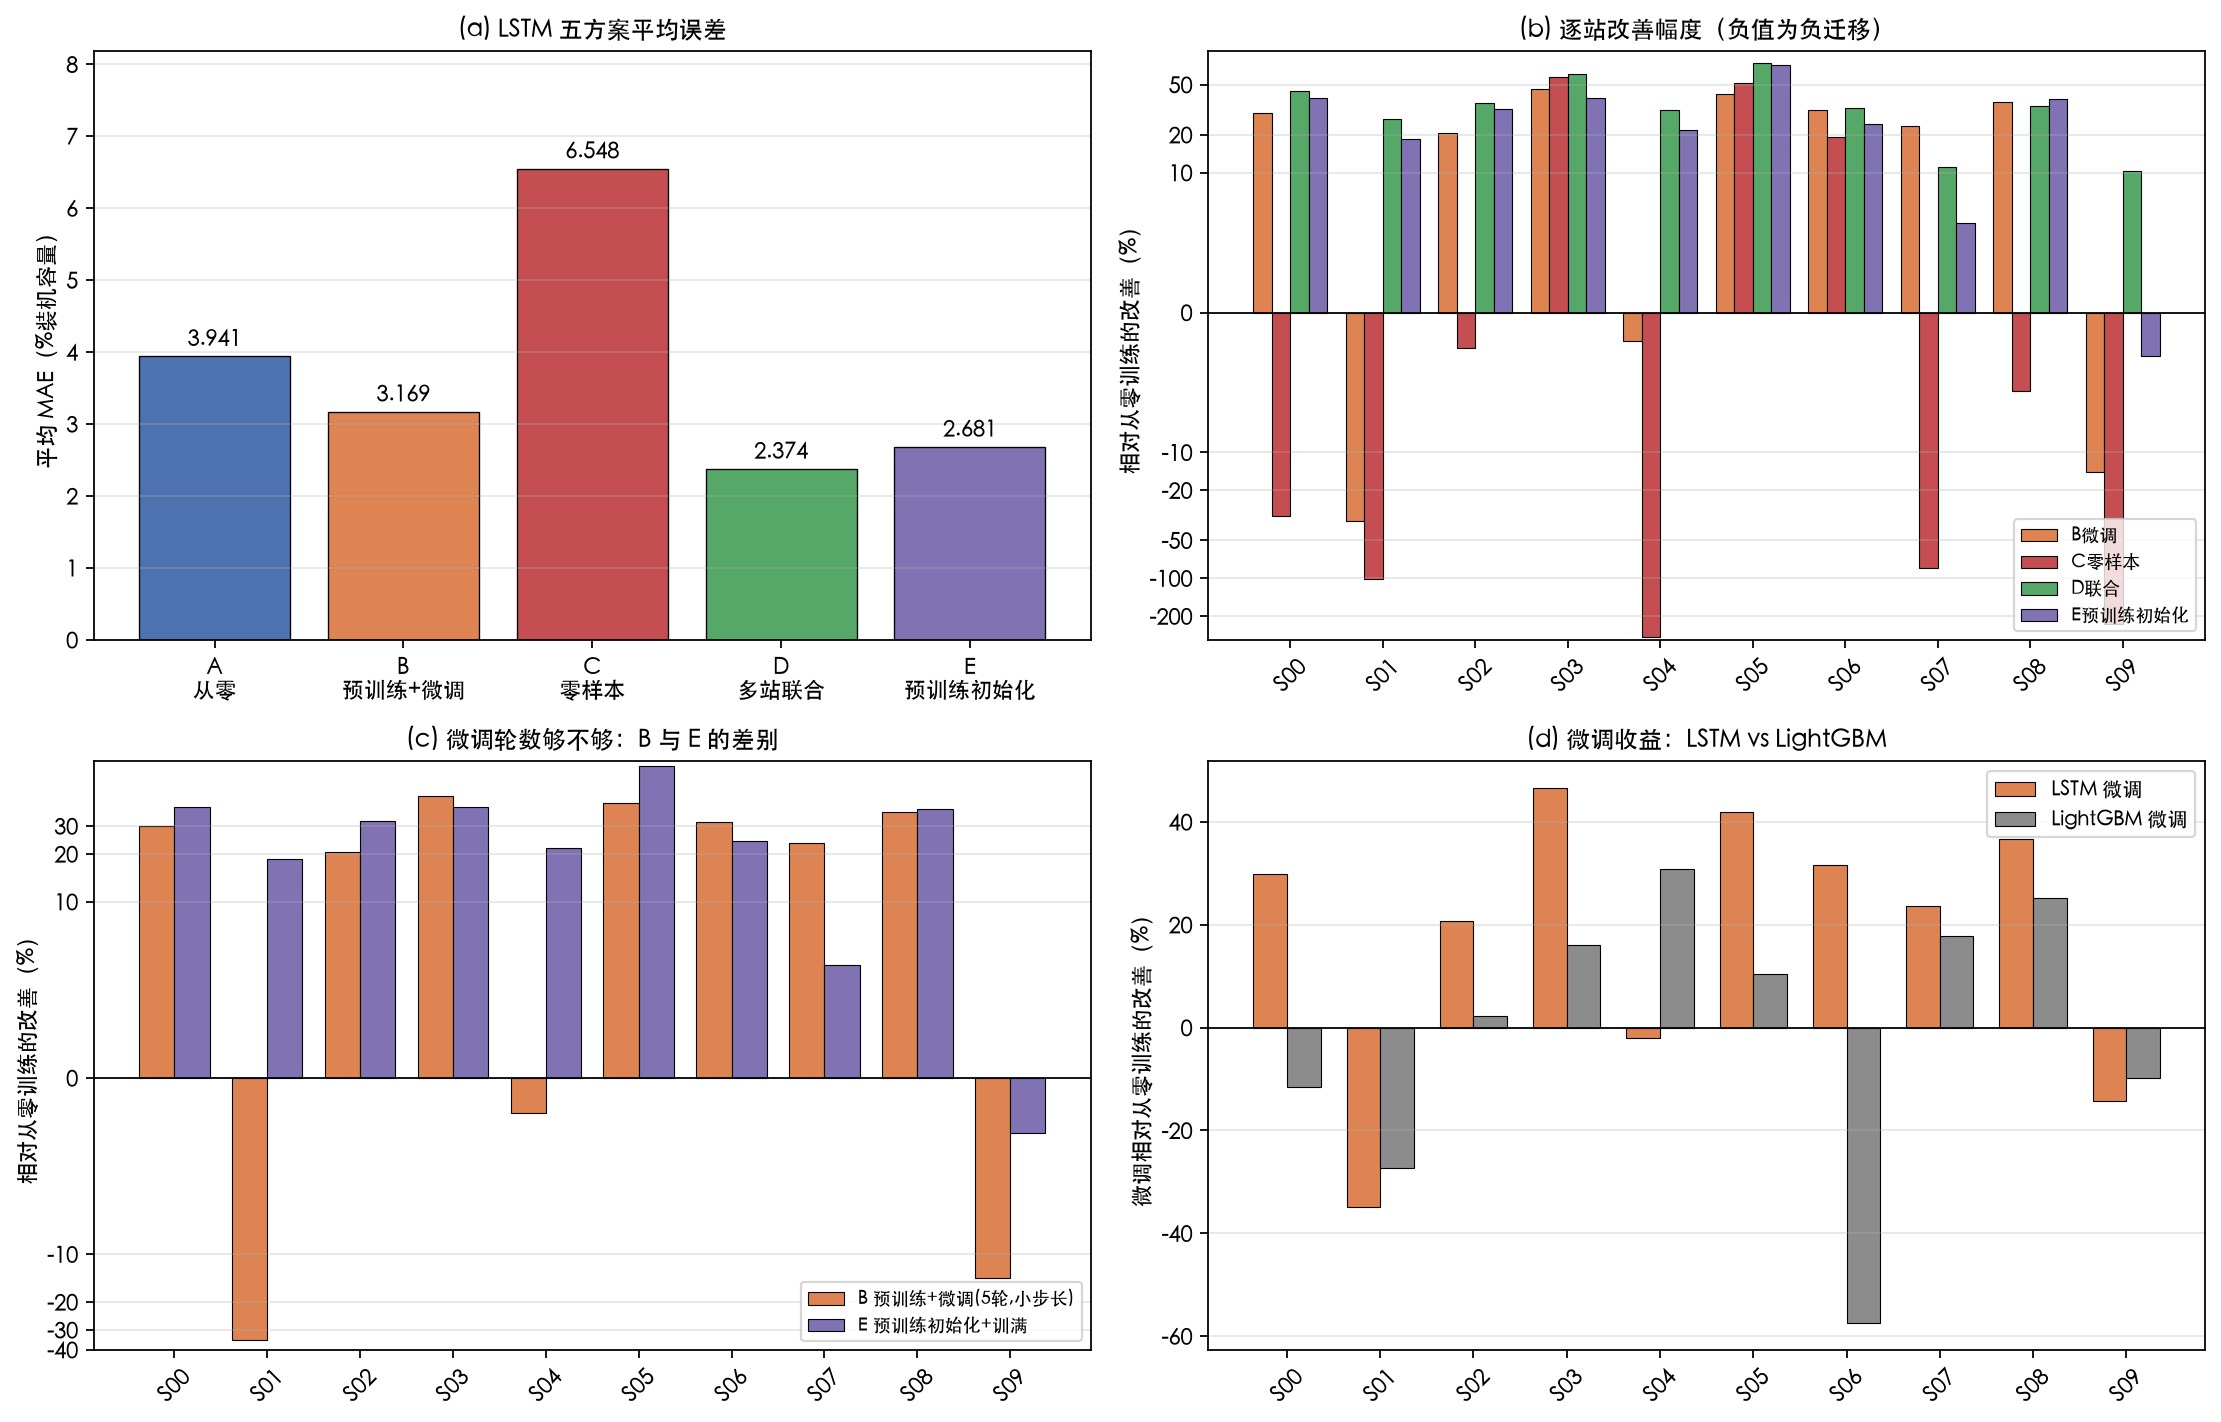
\includegraphics[width=0.95\textwidth]{fig9_lstm_transfer}
\caption{LSTM 迁移实验结果：（a）五方案平均误差；（b）逐站改善幅度，纵轴为对称对数刻度；
（c）B 与 E 的逐站对比；（d）微调收益与 LightGBM 的对照}
\label{fig:lstm}
\end{figure}

表 \ref{tab:lstm} 的排序是 $D>E>B>A>C$，树模型为 $D>B>A>C$。
两个模型在最重要的一点上完全一致：\textbf{多站联合训练都是收益最大的做法}（LSTM 36.15\%、树模型 14.61\%），
也都远优于「预训练 + 微调」。图 \ref{fig:transfer} 与图 \ref{fig:lstm} 并列可以看出这一点。

差别出现在 B 上。树模型的「预训练 + 微调」几乎无效（$-0.36\%$），
LSTM 上却把误差降低 18.01\%、七个站有效。原因在于两种模型「怎么改」不一样：
LSTM 微调时梯度会流回全部权重，预训练学到的时序结构可以被目标站的数据按需重写，
于是「先预训练再微调」这套做法能真正兑现；树模型的微调只能在老树上继续加，
改不动既有结构，因此同样思路在树模型上失灵。

但不能据此说 LSTM 更强。LSTM 从零训练的基线本身就差得多（3.941 对 2.744），
表 \ref{tab:lstm} 里每个方案的绝对误差也都高于表 \ref{tab:transfer} 中对应的树模型；
它看起来「提升幅度大」，很大程度上是起点低、可提升空间大。
准确的表述是：在同一组方案里，可微模型能靠微调拿到收益，树模型拿不到；
而两者共同的、收益也最大的做法，都是直接做多站联合训练。

第二处发现与直觉相反：E 比 D 低 7.2 个百分点（28.96\% 对 36.15\%），
且 E 的站间波动大于 D。说明预训练给出的起点只有在少轮数、小步长下才保得住；
一旦按常规步长训满，源站学到的通用结构会被较快覆盖，也就是灾难性遗忘。
这一点在单站试跑时曾给出相反的信号（当时 E 优于其余方案），把十站跑完才翻转。
单站结论不足为凭，这也是本文坚持用留一站交叉验证的原因之一。

零样本迁移在 LSTM 上更不可用：平均变差 61.45\%，只有 3 个站有效，
station04 上 MAE 从 6.348 恶化到 24.776。两个模型都指向同一个结论——
不校准地直接搬用别站模型风险很大，区别只是神经网络对输入分布的偏移更敏感。

\begin{figure}[htbp]
\centering
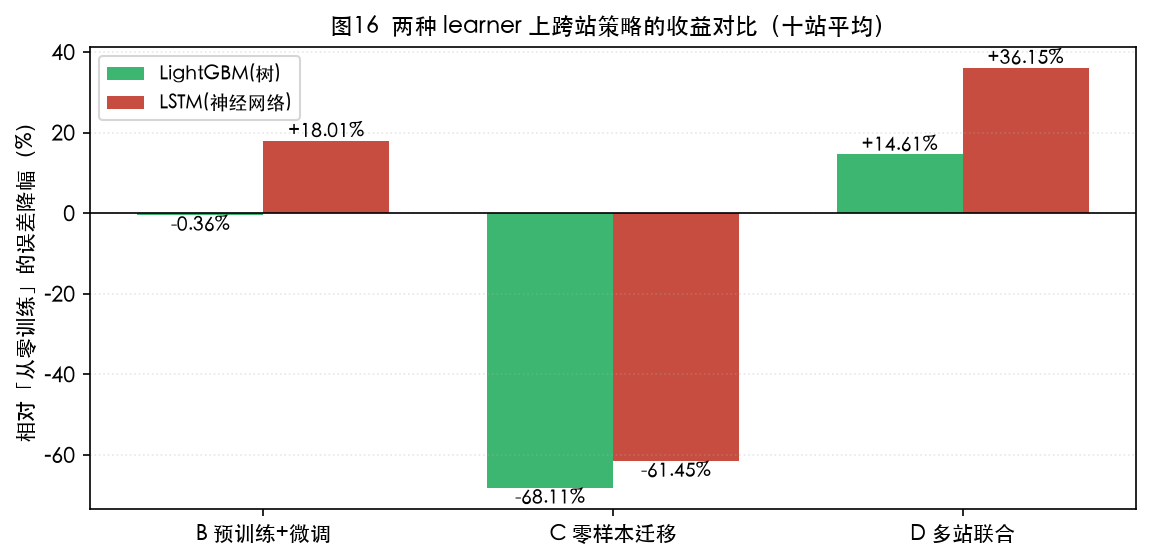
\includegraphics[width=0.94\textwidth]{fig16_transfer_compare}
\caption{两种 learner 上跨站策略的收益对比（相对「从零训练」的误差降幅，十站平均；
零样本迁移为负收益）}
\label{fig:transfercompare}
\end{figure}

图 \ref{fig:transfercompare} 把两类模型的结果并列在一起：柱子在 D 处同时最高，
说明「多站联合训练」是两种 learner 共同的最优解；而在 B 处两根柱子一高一低，
正是「树模型加不了树、神经网络能改写权重」这一差别的直观体现。

\subsection{XGBoost 上的迁移复现（拓展四补充）}
\label{sec:xgb}

上面两节的迁移实验有一个容易被人挑刺的地方：树模型只用了 LightGBM 一种。
\ref{sec:transfersetup} 节交代过，四种做法统一以 LightGBM 实现；
而 \ref{sec:overall} 节的主实验里，树模型是 LightGBM 与 XGBoost 一起跑过的。
若「多站联合训练最优」这条结论只有一类树模型撑着，说到底是欠一次复现。

本文用一个单独的脚本（\texttt{code/24\_xgb\_transfer\_loso.py}）补上这一步：
把 learner 换成 XGBoost，数据与切分口径一字不改地重跑十站的 A/B/C/D 四个方案。
超参按等价口径对齐——\texttt{num\_leaves=31} 取 \texttt{max\_depth=5}
（31 叶的满二叉树深度就是 5），\texttt{min\_data\_in\_leaf=20} 取 \texttt{min\_child\_weight=20}，
bagging 与特征子采样都仍是 0.85，A 仍为 700 棵、B 仍是 500 棵预训练加 200 棵微调，
以免出现「树多所以赢」的比较不公。

表 \ref{tab:xgbtransfer} 给出十站平均结果。排序是 $D>A>B>C$：
多站联合训练把误差压低 4.11\%（6/10 站），
从零训练 2.619 次之，而预训练加微调反而把误差抬高 11.81\%（只有 5 个站有效），
零样本迁移平均恶化 91.32\%，是四个方案里最差的，只有 2 个站不比从零差。
零样本之所以崩得这么厉害，主要被两个站拖住：station04 从 5.909 涨到 10.391，
station09 从 2.689 涨到 10.265——本站特征分布一旦与源站的 9 站整体差得远，
别站训出来的树在原封不动搬过来时误差会成倍放大。

与 LightGBM 逐方案对照（图 \ref{fig:threelearner}），三个策略上两种树模型
的方向完全一致：D 都是正收益、C 都是大幅负值、B 都不成立。
量级上 XGBoost 明显弱于 LightGBM——D 只降 4.11\%（对 14.61\%），
C 恶化 91.32\%（对 68.11\%），B 的 $-11.81\%$ 也比 $-0.36\%$ 更差。
这种差别来自两个库的实现细节而非机制本身，两者都是梯度提升树、都是增量建树，
因此不宜把「提升几个百分点」当作树模型的固有性质，也不必为它做额外解释。
但六次比较（三个策略 $\times$ 两种树模型）的符号全同，
足以说明 \ref{sec:transfer} 与 \ref{sec:lstm} 两节得到的结论不是 LightGBM 一家偶然：

\begin{enumerate}
\item \textbf{多站联合训练始终排第一}——三种 learner 上都是它，
所以在三类模型上都可以放心地把它当作默认做法；
\item \textbf{零样本迁移始终最差}——三种 learner 上都大幅为负，
「直接搬别站模型」在任何一类模型上都行不通；
\item \textbf{「预训练 + 微调」只在可微模型上成立}——LSTM 上 $+18.01\%$，
两类树模型上分别为 $-0.36\%$ 与 $-11.81\%$，
把这条判据和「模型能不能反向传播」绑在一起看，比记具体数字更可靠。
\end{enumerate}

需要如实交代的是：XGBoost 上联合训练的收益比 LightGBM 小得多（10 个站里只有 6 个改善，
station09 上甚至从 2.689 变成 3.001 略有变差）。这说明多站联合的\textbf{有效性}稳，
\textbf{收益大小}会随实现与超参浮动。工程上更稳妥的表述是「联合训练方向可靠、
量级要按自己的数据和求解器实测」，而不是照抄某个百分比。

\begin{table}[htbp]
\centering
\caption{XGBoost 上留一站交叉验证的十站平均结果；表内「相对 A 的改善」为逐站算出后再取平均，与 MAE 列的十站平均口径略有差异。}
\label{tab:xgbtransfer}
\begin{tabular}{lccrc}
\toprule
方案 & MAE & RMSE & 相对 A 的改善 & 优于 A 的站数 \\
\midrule
A 从零训练      & 2.619 & 5.453  & ---         & ---   \\
B 预训练 + 微调 & 2.671 & 5.560  & $-11.81\%$  & 5/10  \\
C 零样本迁移    & 4.962 & 8.980  & $-91.32\%$  & 2/10  \\
D 多站联合训练  & \textbf{2.416} & \textbf{5.100} & \textbf{+4.11\%} & \textbf{6/10} \\
\bottomrule
\end{tabular}
\end{table}

\begin{figure}[htbp]
\centering
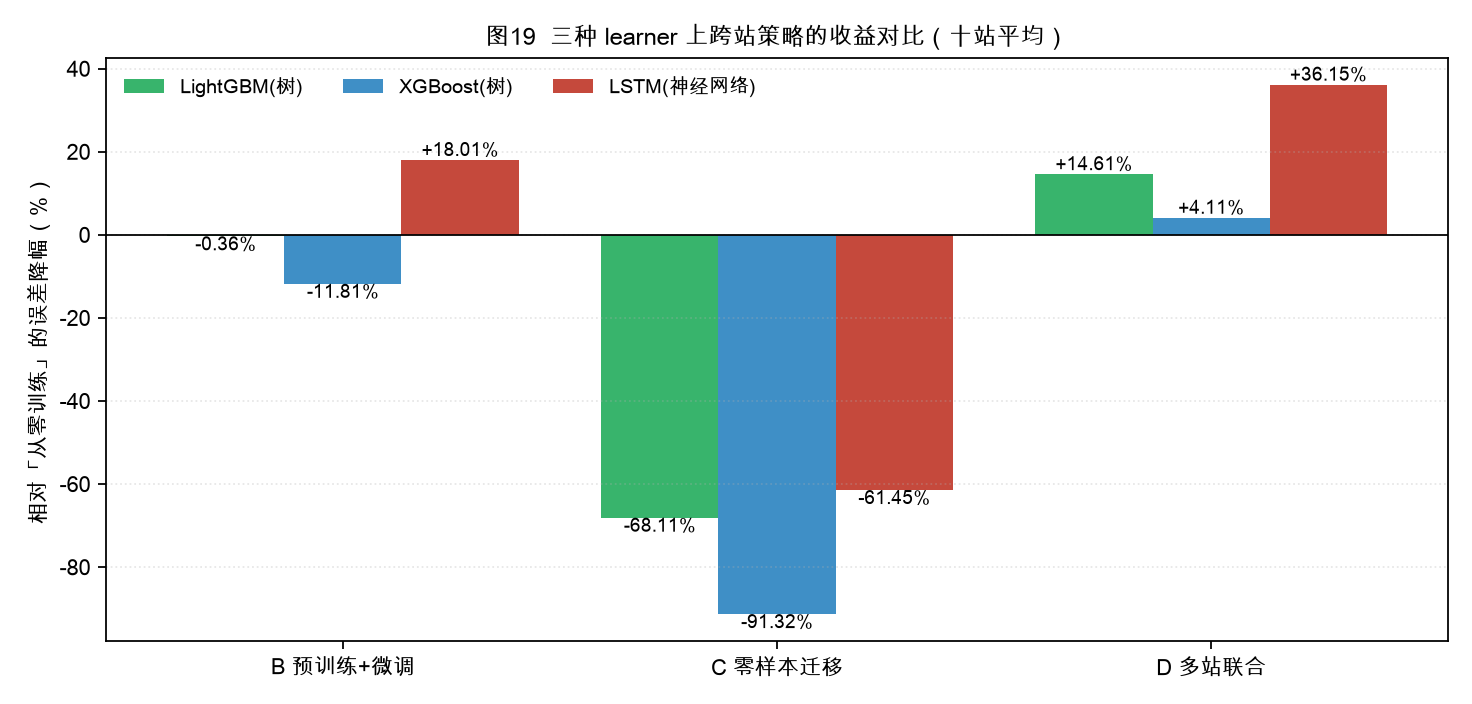
\includegraphics[width=0.94\textwidth]{fig19_three_learner}
\caption{三种 learner 上跨站策略的收益对比（相对「从零训练」的误差降幅，
十站平均；零样本迁移为负收益）}
\label{fig:threelearner}
\end{figure}

\subsection{关于目标列性质的检验}
\label{sec:targetcheck}

在数据取舍阶段，本文对 PVOD 的目标列做过一项性质检验，以确认它是真实计量值而非换算量。
做法是把每条记录的出力与同一时刻实测总辐射作比值，只取总辐射大于 50\,W/m$^2$ 的白天样本，
考察该比值是否恒定，以及控制辐射之后它是否还与气温有关。结果见表 \ref{tab:target}。

\begin{table}[htbp]
\centering
\caption{PVOD 目标列性质检验（十站，白天样本）}
\label{tab:target}
\begin{tabular}{lccc}
\toprule
检验量 & 十站范围 & 十站平均 & 对照：宁夏数据集 \\
\midrule
出力/辐射 比值的变异系数 CV & 19.40\% $\sim$ 58.97\% & 29.69\% & 0.23\% \\
出力与辐射的相关系数        & 0.8889 $\sim$ 0.9785   & ---     & 1.0000 \\
比值与气温的偏相关（控制辐射后） & $-0.5202 \sim 0.5726$ & 0.0730 & 0.0038 \\
\bottomrule
\end{tabular}
\end{table}

两点结论。其一，PVOD 的出力与辐射相关虽高（0.8889$\sim$0.9785），但明显不是完美的线性关系：
比值自身的变异系数在十站落在 19.40\%$\sim$58.97\%，平均 29.69\%，
与宁夏数据集的 0.23\% 相差约 130 倍。这说明 PVOD 的出力保留了真实运行中的各种波动——
云层遮挡、限发、组件污渍、逆变器效率变化等，是独立计量的电表读数。

其二，控制辐射后，比值与气温的偏相关在十站之间符号并不一致（$-0.5202$ 到 $+0.5726$，
平均 $0.0730$），对应的温度效应为 $-1.29 \sim +1.66\ \%/^{\circ}\mathrm{C}$，平均 $+0.20\ \%/^{\circ}\mathrm{C}$。
理论上组件温度升高会降低效率，该效应应为负；十站平均却是正的，且站间符号混乱。
本文的解释是：温度效应确实存在，但它在本数据中被限发（station09）、容量登记错误（station04）等
未观测因素以及辐射的共线关系掩盖，单凭这份数据无法把它干净地分离出来。
这也与 \ref{sec:ablation} 节消融实验「温度特征不带来可测增益」的结果互相印证。

综合来看，PVOD 的目标列可作真实出力使用，本文所有结论均基于此。而宁夏那份数据
因其目标列近似为辐射的固定倍数换算值（CV 仅 0.23\%）、且缺经纬度与装机容量，
无法完成容量归一化与跨站比较，故本文全部实验改用 PVOD。

% ============================================================
\subsection{误差的分方向统计与工程代价折算}
\label{sec:errordir}

前面用到的 MAE、RMSE 都是对称指标：把正误差和负误差取绝对值之后一起平均，
只知道「差多少」，不知道「差在哪一边」。可第~\ref{sec:concl} 节说的工程代价恰恰是有方向的。
本节把预测误差按方向拆成两半——定义 $e(t)=\hat{P}(t)-P(t)$，
$e<0$ 记为\textbf{少报}（预测偏低，实际发多了），$e>0$ 记为\textbf{多报}（预测偏高，实际发少了），
分别统计两侧的电量，再乘上真实电价折算成钱。

\emph{价格锚点全部取自公开文件}，不用估算。弃光电量按河北南网 2025 年光伏结算均价
0.3433\,元/kWh 计（冀南全年光伏结算电量 83.96 亿\,kWh 的加权均价）；
缺额电量按河北南网燃煤发电基准价 0.3644\,元/kWh 计，这也是存量新能源机制电价的执行基准
\cite{hebei_pricing}；做敏感性检验时取河北南网现货市场出清上限 1.2\,元/kWh
（2025 年 3 月 1 日起连续结算试运行）\cite{hebei_spot}。
这里先按\emph{全额兑现的上界}计算，即假定每个断面的方向性偏差都真实转化成了弃电或缺额，
实际调度有吸收能力，真实代价只会更低。

表 \ref{tab:errdir} 给出十站在测试期（约 85 天、4.9 万个有日照的断面）的合计。

\begin{table}[htbp]
\centering
\caption{误差两个方向的电量与代价（十站测试期合计，全额兑现上界）}
\label{tab:errdir}
\begin{tabular}{lrrrr}
\toprule
预测方案 & 少报电量 & 少报代价 & 多报电量 & 多报代价 \\
 & (万\,kWh) & (万元) & (万\,kWh) & (万元) \\
\midrule
甲$'$ 预报气象 + Persistence  & 630.55 & 216.47 & 1540.12 & 561.22 \\
甲$'$ 预报气象 + 线性回归      & 675.76 & 231.99 & 1412.63 & 514.76 \\
丙 实测气象 + LightGBM       & 432.20 & 148.37 & 203.67  & 74.22  \\
丙 实测气象 + 线性回归        & 308.54 & 105.92 & 223.83  & 81.56  \\
丙 实测气象 + Persistence     & 486.69 & 167.08 & 486.07  & 177.12 \\
\bottomrule
\end{tabular}
\end{table}

图 \ref{fig:errdir} 是同一组数据的柱状对照。

\begin{figure}[htbp]
\centering
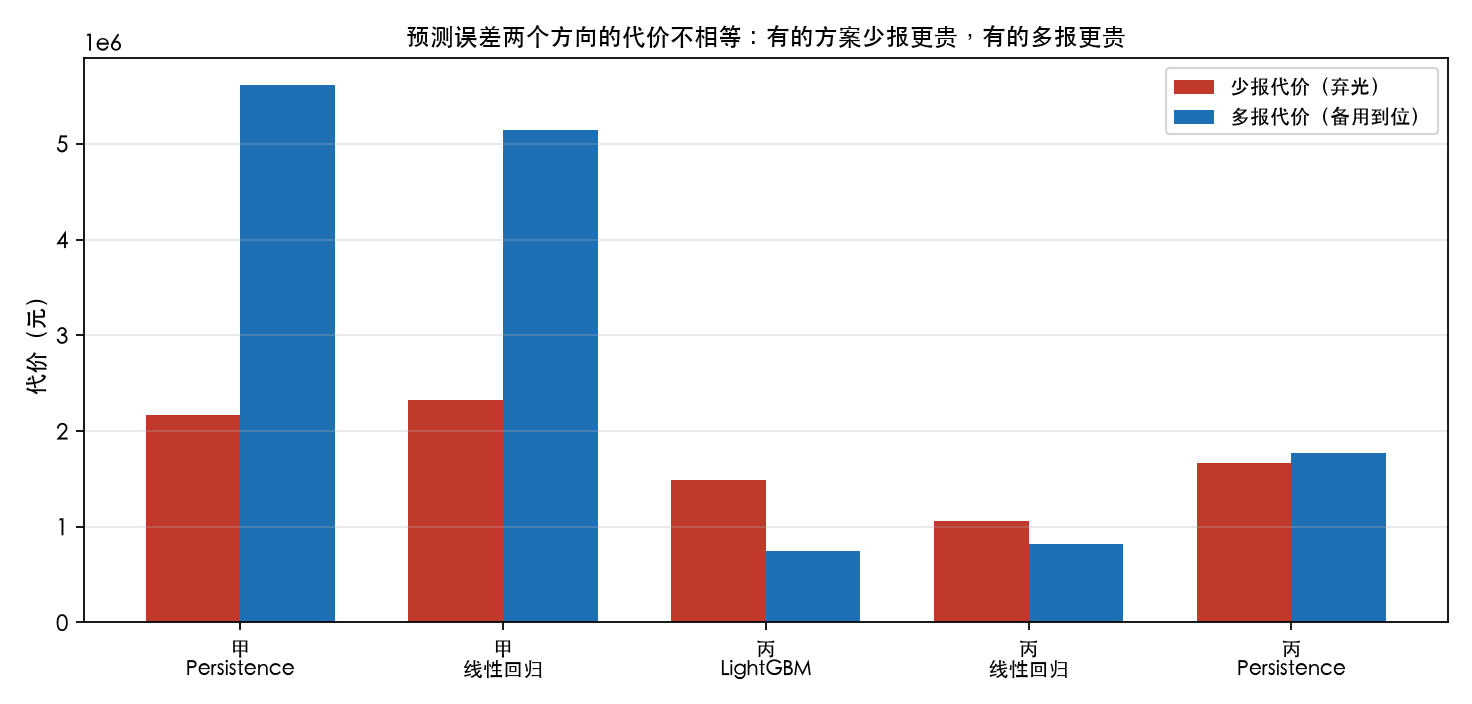
\includegraphics[width=0.82\textwidth]{fig17_error_direction.png}
\caption{少报代价（弃光）与多报代价（备用缺额）并不相等：
设定甲$'$ 以多报为主、设定丙以少报为主，风险方向整个翻了过来。}
\label{fig:errdir}
\end{figure}

结论先说清楚：**把信息源从「数值预报」换成「站内实测」，风险的主要方向被整个翻了过来。**
设定甲$'$ 上多报代价是少报的 2.6 倍（561.22 万元对 216.47 万元），钱主要花在
「预测偏高、实际发不出来」这一侧；到了设定丙，LightGBM 反过来以少报为主，
少报代价 148.37 万元是多报 74.22 万元的 2.0 倍；而 Persistence 基线两侧几乎相等（167.08 对 177.12），
说明它压根不偏，只是都差。这个翻转在 MAE 上看不见——
两个设定的 MAE 相差约 3 倍（$4.87\%$ 对 $1.64\%$），但即便只看总量，也看不出风险是往哪边倒的。

少报也不是均匀撒在各处的。表 \ref{tab:errbin} 把设定丙下 LightGBM 的误差按同时刻总辐射分档，
图 \ref{fig:errbin} 是同一组数据的柱状图。

\begin{table}[htbp]
\centering
\caption{设定丙 LightGBM 的误差按同时刻总辐射分档（十站测试期合计）}
\label{tab:errbin}
\begin{tabular}{lrrr}
\toprule
总辐射 GHI (W/m$^2$) & 断面数 & 少报电量 & 多报电量 \\
 & & (万\,kWh) & (万\,kWh) \\
\midrule
$0\sim50$     & 11014 & 59.32  & 5.80  \\
$50\sim300$   & 13200 & 61.73  & 45.39 \\
$300\sim600$  & 9725  & 80.43  & 66.98 \\
$600\sim1000$ & 12800 & 163.76 & 72.16 \\
$>1000$       & 2294  & 66.95  & 13.33 \\
\bottomrule
\end{tabular}
\end{table}

\begin{figure}[htbp]
\centering
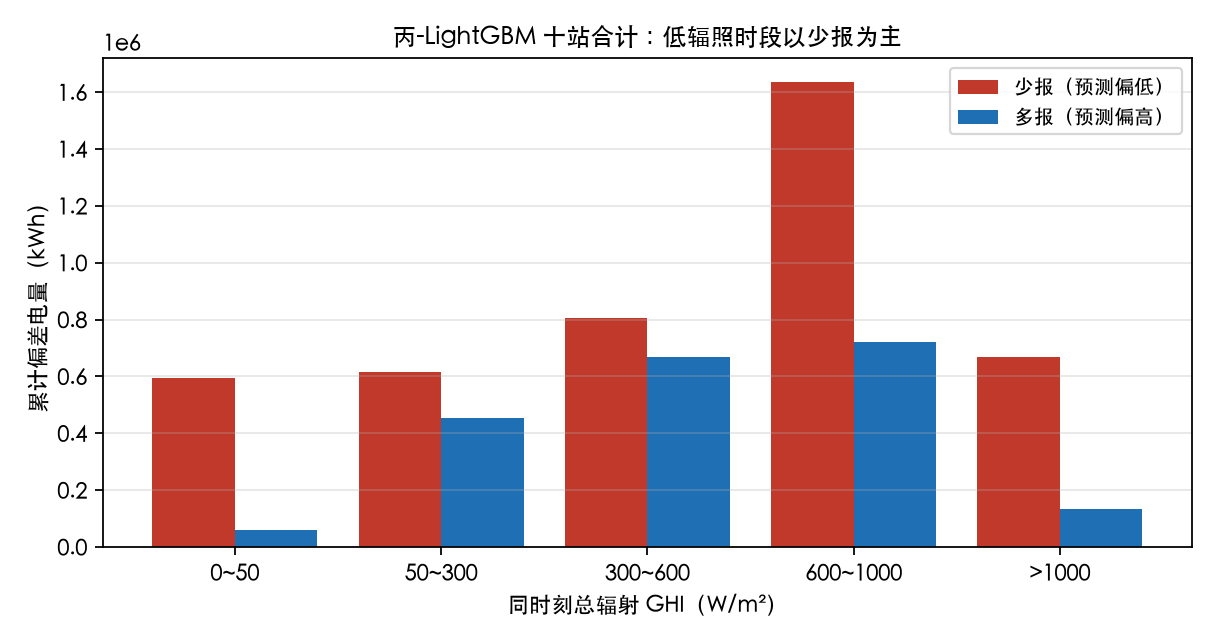
\includegraphics[width=0.74\textwidth]{fig18_error_by_irradiance.png}
\caption{少报（预测偏低）随辐射增强而增大，强辐照时段是弃光的主要风险源。}
\label{fig:errbin}
\end{figure}

两点值得注意。其一，$600\sim1000$\,W/m$^2$ 这一档单独贡献了 38\% 的少报电量，
而它正是全天出力最大、最容易装不下的时段——也就是说，
真正的弃光风险不是出现在阴天，而是出现在\emph{晴天正午预测偏保守}。
其二，$0\sim50$\,W/m$^2$ 档的少报/多报比高达 10.2:1，是最偏的一档，
但该档绝对量只有 $600\sim1000$ 档的三分之一，量级上不足以主导总代价。

既然少报更贵，直觉上「把预测整体抬高一点点」应该能省钱：多报只是略贵
（0.3644 对 0.3433，仅差 6\%），少报一点基本不亏，少掉的少报却是净赚。
本文真的在 $\delta\in[-3\%,+3\%]$ 上逐点重算总代价扫了一遍，结果见表 \ref{tab:biascal}。

\begin{table}[htbp]
\centering
\caption{整体偏置 $\delta$ 的扫描（$\delta>0$ 表示把预测整体抬高）}
\label{tab:biascal}
\begin{tabular}{lrrr}
\toprule
预测方案 & 主口径最优 $\delta$ & 主口径节省 & 现货上限口径节省 \\
\midrule
丙 实测气象 + Persistence    & $+0.0$\% & 0.00\%  & 0.63\% \\
丙 实测气象 + 线性回归       & $+1.3$\% & 0.01\%  & 1.47\% \\
丙 实测气象 + LightGBM       & $+0.3$\% & 0.00\%  & 1.14\% \\
甲$'$ 预报气象 + Persistence  & $-3.0$\% & 0.18\%  & 0.43\% \\
甲$'$ 预报气象 + 线性回归     & $-3.0$\% & 0.26\%  & 0.53\% \\
\bottomrule
\end{tabular}
\end{table}

这是一条\emph{负面结果}，但比正面结果更有用：**这条路基本走不通。**
主口径下最优偏置只有 $+0.3\%$（丙 LightGBM），节省 0.00\%；
把多报单价换成现货出清上限 1.2\,元/kWh 再扫，最优偏置落到 $-3\%$ 的扫描边界，
节省也不过 1.14\%。原因不难想见——两个方向的单价只差 6\%，
靠挪动整体偏移量赚不回来。真正省钱的是换信息源而非调偏置：
同样这 85 天里，甲$'$ 的总代价 777.69 万元，丙 LightGBM 只有 222.59 万元，省 71.4\%。

一处必须交代的口径局限：表 \ref{tab:biascal} 里的 $\delta$ 是在\emph{测试期}上扫出来的，
工程上属于拿测试数据调参，会高估收益；真实部署应该用独立的滚动校准窗口按日更新 $\delta$。
本节也只统计了方向性偏差，没有考虑偏差的时间累计效应（例如连续多时段少报会不会触发不同的调度规则）。

% ============================================================
\section{结论}
\label{sec:concl}

本文基于河北十座光伏电站的公开数据集 PVOD（271968 条、15 分钟粒度），
比较了「同时刻站内气象可得」「同时刻仅有数值天气预报」「仅历史观测可用」以及
「同时刻气象与历史观测兼有」四种信息条件下的光伏短时出力预测效果，
并检验了结论的跨站可迁移性，最后把预测误差按方向拆开、按真实电价折算成工程代价。
主要结论有八点：

\begin{enumerate}
\item 信息条件比模型选择更决定精度。同时刻实测气象加历史观测时，最优 MAE 为 1.4942\%；
只去掉同时刻气象（设定乙）即升至 2.2821\%；把同时刻实测气象换成数值天气预报（设定甲$'$）则为 4.8725\%，
约为实测条件下的两倍。可见接入一条实时气象实测，比换更复杂的模型更划算。

\item 在最有利条件（设定丙）下，表现最好的竟是线性回归，而非任何树模型：
MAE 1.4942\%、$R^2$ 0.9849，优于第二名的 LightGBM 8.8\%、优于 Persistence 基线 41.74\%。
专门做的恒等映射检验给出了机制解释——Persistence 本质是硬编码的 $P(t)=1.0\times P(t-1)$，
线性回归能学到接近 1 的系数（十站平均 0.9788）从而复现它，而随机森林只能输出叶内均值，
单独使用该特征时反而比 Persistence 差 22.90\%。这提示在含强自回归项的预测任务中，
线性基线必须与树模型并列比较。

\item 模型增益高度依赖天气动态。辐射突变 30$\sim$60\,W/m$^2$ 与超过 60\,W/m$^2$ 时降幅分别为
14.54\% 与 17.90\%，而辐射平稳（$<$10\,W/m$^2$）时段随机森林反而比 Persistence 差 163\%。
Persistence 是平稳天气下的天然强基线，实际使用宜按辐射突变强度切换预测策略。

\item 同时刻气象的贡献不可被历史信息替代：设定丙中把 6 个同时刻气象变量整组删除后，
MAE 恶化 61.49\%。相反，气温、气压、风速等次要气象因子删掉后误差几乎不变（0.19\%），
时刻编码的贡献也只有 0.09\%。但这是信息冗余，不代表温度对光伏没有物理影响。

\item 针对研究问题一——复杂模型并不必然更好。把 LSTM 放进与树模型完全相同的条件下，
它在四个设定上\textbf{全部落后}：设定甲 3.1467 对最优树模型 2.4738（差 27.2\%），
设定丙 3.1624 对线性回归 1.4942（差 111.6\%），
设定乙里甚至输给完全不需要训练的 Persistence 基线 61.6\%。
训练代价上，单站 LSTM 约需 9.6 秒，是线性回归（0.003 秒）的三千余倍，精度却更差。
本文给出三点解释：本任务的出力与同时刻辐射近似瞬时映射，几乎不需要长程记忆；
每站 1$\sim$3.3 万条记录对神经网络偏小；且夜间零出力样本占 49.07\%，
与白天的规律完全不同，LSTM 必须用一套权重同时学会两种模式。
这说明在这类表格型回归任务上，先把朴素基线与树模型做到位，比直接上深度模型划算。

\item 针对研究问题二——跨站迁移值得做，而且最佳做法在三类模型上是一致的，
都是\textbf{多站联合训练}：树模型上降低误差 14.61\%（8/10 站）与 4.11\%（6/10 站），
LSTM 上降低 36.15\%（10/10 站），各自都是本组方案里最优的。
两者的差别只出现在「预训练 + 微调」上：树模型上无效甚至有害（$-0.36\%$ 与 $-11.81\%$），
因为它只能在既有的 500 棵树上继续加树、改不动旧结构；
LSTM 上则有效（18.01\%、7/10 站），因为梯度会流回全部权重，预训练学到的结构可被按需重写。
换第二棵树（XGBoost）复跑后，三个策略上两类树模型的方向全同，
说明上述判据不是某一个库的偶然，而「收益大小会随实现浮动」
（同一策略上 14.61\% 与 4.11\% 相差十余个百分点）才是需要交代的界限。
此外 LSTM 上「预训练初始化后按常规步长训满」只得 28.96\%，不如多站联合的 36.15\%，
说明预训练给出的起点会被后续训练覆盖，需要在少轮数、小步长下才保得住。
注意 LSTM 的绝对误差仍全面高于树模型，其「提升幅度大」主要源于起点低、可提升空间大。

\item 零样本迁移在两类模型上都不宜直接使用：树模型平均变差 68.11\%、仅 3/10 站有效；
LSTM 平均变差 61.45\%、同样仅 3/10 站有效。两者都指向同一结论——
不校准地搬用别站模型风险很大，区别只在神经网络对输入分布的偏移更敏感。
真正有效的是把别站数据作为\textbf{训练素材}而非\textbf{现成模型}来使用。

\item MAE 的对称性，与工程成本的非对称性，是可以量出来对账的。
按河北南网真实电价折算（弃光 0.3433\,元/kWh、缺额 0.3644\,元/kWh），
十站测试期 85 天的代价以两个设定为例：设定甲$'$ 以\textbf{多报}为主（561.22 万元对 216.47 万元，2.6 倍），
设定丙则以\textbf{少报}为主（148.37 万元对 74.22 万元，2.0 倍）——
换一个信息源就把风险的主要方向整个翻了过来，这是任何对称指标都看不出来的。
而且少报集中在 $600\sim1000$\,W/m$^2$ 的强辐照时段（占全部少报电量的 38\%），
恰好是出力最大、最容易装不下的时段，弃光风险正落在这里。
本文还试过一种更省事的优化——给预测整体加一个常数偏置，
主口径下几乎零收益（$\le0.26\%$），改用现货出清上限 1.2\,元/kWh 计价也只省 1.14\%，
而换信息源能省 71.4\%：对这类任务，事后调偏置不值得花力气，
该花的功夫在把气象数据接对。

\end{enumerate}

\noindent\textbf{工程应用含义。}预测精度最终要落到电网运行的代价上，
而\emph{这个代价是有方向的}：同样的误差大小，往哪个方向偏，后果并不一样。
光伏电站需要按规定向调度上报功率预测曲线，调度据此决定常规机组的开机组合与旋转备用容量
\cite{inman2013solar}。

\textbf{少报（预测值低于实际出力）主要损失的是电量。}
调度按偏低的预测多开了常规机组，实际光伏却发得更多，系统出现出力过剩；
而火电机组受最小技术出力约束，不能无限制往下压，多余的光伏电量往往只能弃掉，
结果就是清洁电力被白白浪费、消纳率下降。

\textbf{多报（预测值高于实际出力）主要损失的是金钱。}
调度按偏高的预测压减了常规机组，实际光伏发不出来，系统出现功率缺额，
只能靠旋转备用、储能放电或快速启停机组临时顶上，这部分电量的成本远高于正常发电，
严重时还会威胁频率稳定，并按并网考核规则产生偏差考核费用。

两个方向都不可忽略，且后者的单位代价通常更高——少掉的电「不值钱」，
临时补上的电「很贵」。

这个非对称性不是嘴上说说，第~\ref{sec:errordir} 节已经把它量化了对账：
按河北南网的真实电价把十站测试期的误差折算成钱，
设定甲$'$ 花掉 777.69 万元而其中 72\% 是\textbf{多报}造成的，
设定丙花掉 222.59 万元而其中 67\% 是\textbf{少报}造成的。
两个设定的 MAE 相差约 3 倍（$4.87\%$ 对 $1.64\%$），但真正决定「钱花在哪一边」的，
是误差偏向哪一侧、以及偏向的那侧单价有多高。
因此工程上报告误差时，只给一个 MAE 是不够的，至少应该同时给出偏置（bias）与两侧的代价。

把这条链条再往上推一层，就接到「双碳」目标上：
预测越不准，调度越不敢少留备用，系统就必须在光伏大发时段也维持一批随时可上调的火电容量兜底，
这部分容量即使大部分时间闲置，也要保持热态、持续产生排放；
反过来，把预测误差压下去，一头能减少这种「为防不确定而多留的火电」，
另一头能减少弃光、提高清洁电量的占比，两边都直接服务于碳减排。
因此提高预测精度不只是电站侧的一笔经济账，它同时也是电网侧的减碳手段。

本文的数字可以给出一个直观的量级。十站总装机 193.6\,MW（平均单站 19.36\,MW，取自数据集配套元数据）：
设定甲接入站内实测气象时 MAE 为 2.4738\%，相当于每个 15\,min 断面平均有约 4.79\,MW 的偏差
需要靠备用或调节手段去填（单站约 0.48\,MW）；若改用数值天气预报（设定甲$'$），
误差升到 4.8725\%，同一数字变为约 9.43\,MW（单站约 0.94\,MW），二者相差约 4.64\,MW。
这 4.64\,MW 就是「接一条站内实测气象」所对应的备用缺口规模，
说明第~\ref{sec:overall} 节那几个百分点在工程中是有具体功率含义的。

落到实际部署上，本文结果给出四条建议：
一是若电站配有气象站，应优先把实时辐射数据接入预测系统，其收益远大于升级算法；
二是预测策略宜按天气动态分档——云层扰动时段交给机器学习模型，
晴朗平稳时段直接用 Persistence 反而更稳，还能省下算力；
三是新建电站数据不足时，把周边已运行电站的数据\textbf{混合进来联合训练}是低成本且有效的做法，
但不要把别站训好的模型直接拿来用（第~\ref{sec:transfer} 节显示零样本迁移在三类模型上都是负收益）；
至于能降多少，第~\ref{sec:xgb} 节的复现说明它取决于所用的树引擎与超参，
应实测一次再定预期，不宜照抄本文的百分比；
四是选型上不必盲目追求深度模型，本文任务里 LSTM 的精度与训练代价全面劣于树模型与线性回归，
先把线性基线与树模型做扎实更划算。

本文存在五点局限：一是仅使用 PVOD 一份数据集的一年记录，虽含十座电站，
但地域集中于河北，结论能否推广到其他气候区未经验证；二是未做超参数搜索，
模型参数取固定值（100 棵、学习率 0.1），最优模型可能尚未被找到；
三是 LSTM 部分只试了单一网络结构与固定轮数（单站对照 30 轮、迁移实验 15 轮），
未搜索层数、隐藏单元与学习率，其绝对误差也高于树模型，
故该组实验只用于比较各方案的相对次序与迁移规律，不宜当作精度上限；
四是 station04 的容量登记与 station09 的限发问题虽已指出，但本文未做进一步的数据修正，
相关站的结论需谨慎对待；五是十座电站同处河北、气候背景相近，
这会让跨站迁移显得更容易奏效，收益能否同样出现在气候差异更大的区域，尚待验证；
六是第~\ref{sec:errordir} 节的代价折算用的是公开电价与「全额兑现」的上界假设，
没有接入实际的调度仿真，真实弃电率与备用调用量取决于电网当时的运行方式与断面约束，
本节数值只能用于判断两个方向的数量级关系，不宜当作电站的真实账单。
后续工作可在多气候区数据上验证本文结论，并尝试在辐射突变临近时引入更长的滚动窗口，
以及把本节的分方向统计接到滚动预测（day-ahead）的考核口径上。

% ============================================================
\section*{参考文献}
% 正文中引用过的文献在此列出，文献条目定义见同目录 refs.bib。
\bibliographystyle{plain}   % 需要 GB/T 7714 样式时改为 gbt7714（需自行上传 .bst）
% 说明：plain 样式下列出的英文条目标题偏长，编译时会有一行轻微
% underfull \hbox 提示（badness 1082，不影响排版效果与 PDF 生成），
% 已核对过不是缺字或断行错误，故未强行用 \sloppy 掩盖。
\bibliography{refs}

\end{document}

